% $Id$

In this chapter, we use the techniques developed in the previous chapters to
to search for gravitational waves from binary black hole MACHO inspiral in
data from the second LIGO science run.  The goal of the search is to detect
the gravitational waves emitted by the late stages of inspiral. In the absence
of detection, however, we may place an \emph{upper limit} on the rate of
inspiralling BBHMACHOs which may be compared this to the predicted rate of $5
\times 10^{-2} \times 2^{\pm 1}$ discussed in chapter \ref{ch:macho}.  In
section \ref{s:s2run} we describe the data sample used in the analysis.
Section \ref{s:s2tuning} describes how the parameters of the search listed in
the previous chapter were tuned on the playground data. Section \ref{s:monte}
described the Monte Carlo simulations used to measure the efficiency of the
pipeline. In section \ref{s:s2background} we describe the background
observed in the S2 data.

Analysis of the full S2 data set for gravitational waves from inspiralling
BBHMACHOs is complete and the result of this search will appear in
\cite{S2Macho:2004}. Since this result is currently embargoed pending LIGO
Scientific Collaboration internal review, we instead present the result of the
search on the playground data. No gravitational waves from BBHMACHO inspirals
were found in the playground, so in section \ref{s:s2upperlimit} we compute
an upper limit on the rate of BBHMACHO inspirals in the playground data.
Although this result contains statistical bias, as it is computed from data
used to tune the pipeline, it allows us to make a reasonable prediction of the
upper limit obtained from the full S2 data, assuming no BBHMACHO signals are
detected in the full data set. In which case I'd be in a pub Stockholm, not in
my office at 2am on a Wednesday morning.

\section{The Second LIGO Science Run}
\label{s:s2run}

All three LIGO detectors operated during the second science run, referred to
as S2, which lasted for 59 days (1415 hours) from February 14 to April 14,
2003.  Although the detectors were manned by operators and scimons 24 around
the clock, the amount of data flagged as science mode was limited by
environmental factors (especially high ground motion at LLO and strong winds
at LHO), occasional equipment failures, and periodic special investigations.
The total amount of science data obtained was 536 hours for L1, 1044 hours for
H1, and 822 hours for H2.

The analysis described in this thesis uses data collected while the LLO
detector was operating at the same time as one or both of the LHO detectors in
order to make use of the triggered search pipeline.  Science mode data during
which both H1 and H2 were operating but L1 was not, amounting to 383 hours,
was not used in this analysis because of concerns about possible
environmentally-induced correlations between the data streams of these two
co-located detectors. This data set, as well as data collected while only one
of the LIGO detectors was in science mode, will be combined with data from the
third LIGO science run in a future analysis. Figure~\ref{f:S2times} shows a
breakdown of the data recorded during S2 by interferometer. The data used in
this search is shown by the shaded region.

As described previously, the noise spectrum of the interferometer affects the
inspiral search pipeline in two important ways. The first is to set the
\emph{sensitivity} of the search, which we can summarize  in terms of the
distance to which an optimally oriented binary system would yield an amplitude
signal-to-noise ratio (SNR) of 8 when extracted from the data using the
matched filtering described in chapter \ref{ch:findchirp}.  The second effect
of the noise curve is on the size of the template bank as described in section
\ref{ss:templatebank}; the greater the sensitivity at low frequencies
(relative to higher frequencies) the larger the template bank.  Since we are
limited in the amount of computational resources available and searching for
lower mass inspirals requires more templates, the noise curve determines what
regions of the mass parameter space it is reasonable to search. These effects
are summarized in figure~\ref{f:inspiral_summary}, which shows the size of the
L1 template bank over the course of the run and the ranges of the three
interferometers to BBHMACHOs.

Template banks were generated at a minimal match of $0.97\%$ from a various
choices of minimum (component) mass up to a maximum component mass of
$1\,M_\odot$. It can be seen that although there is not a significant
fluctuation in the number of templates required for a given lower mass over
the course of the S2 run, there is a large variation in the number of
templates required as a function of lower mass. The scaling of template number
as a function of lower mass is consistent with that described in
\cite{Owen:1998dk}. As described in chapter \ref{ch:macho}, the MACHO mass
range measured by microlensing is $0.15\,M_\odot$ to $0.9\,M_\odot$ at $95\%$
confidence. It would therefore be desirable for the BBHMACHO inspiral search
to cover a region of mass parameter space slightly larger than this, say
$0.1\,M_\odot$ to $1.0\,M_\odot$.  It can be seen, however, that almost an
order of magnitude more templates are needed to decrease lower boundary of
the mass parameter space from $0.2\,M_\odot$ to $0.1\,M_\odot$.  Therefore,
given the computational resources available for the BBHMACHO search, the
lowest mass template in the bank was set to $0.2\,M_\odot$. Note that for the
final search, the match of the template bank was also lowered to $0.95\%$ to
further decrease the number of templates to an average of $14\,179$ over the
S2 run. This can be justified by the sensitivity to galactic BBHMACHOs in S2,
as will be seen below.

The maximum inspiral ranges shown in figure~\ref{f:inspiral_summary} for S2
are consistent with the relative sensitivities of the noise curves. It should
be noted that at no times are either of the LHO interferometers more sensitive
than the LLO interferometer, justifying the triggered search pipeline. In fact
the LLO interferometer has a significantly larger range than either of the LHO
interferometers, at times being sensitive to BBHMACHO inspirals in Andromeda.
Since we require coincidence in L1 and one of the LHO interferometers to make
a detection in this search, however, we are restricted to a search for
BBHMACHOs in the Galactic halo.  

\section{Tuning the Analysis Pipeline}
\label{s:s2tuning}

The entire analysis pipeline was explored first using the playground data set
in order to tune the values of the various parameters. The goal of tuning the
pipeline is to maximize the efficiency of the pipeline to detection of
gravitational waves from binary inspirals without producing an excessive rate
of spurious candidate events.  The detection efficiency $\varepsilon$ is
determined by a Monte Carlo simulation in which we inject simulated inspiral
signals from our model population into the data. The efficiency is given by
the ratio of number of signals detected to the number injected, as described
in the next section.  In the absence of a detection, a pipeline with a high
efficiency and low false alarm rate allows us to set a better upper limit, but
it should be noted that our primary motivation is to enable reliable detection
of gravitational waves. By evaluating the efficiency directly by a Monte Carlo
method in which signals from the hypothetical population are injected into the
data and then sought, we account for any systematic effects caused by the
various vetoes and methods in our pipeline.

There are two sets of parameters that we are able to tune in the pipeline: (1)
the single interferometer parameters which are used in the matched filter and
$\chi^2$ veto to generate inspiral triggers in each interferometer, and (2)
the coincidence parameters used to determine if triggers from two
interferometers are coincident. The single interferometer parameters include
the signal-to-noise threshold, $\rho^\ast$, the number of frequency sub-bands
in the $\chi^2$ statistic, $p$, the $\chi^2$ cut threshold.
and the coefficient on the SNR dependence of the $\chi^2$ cut, $\delta$. These
are tuned on a per-interferometer basis, although some of the values chosen
are common to two or three detectors.  The coincidence parameters are the time
coincidence window for triggers, $\delta t$, the mass parameter coincidence
window, $\delta m$, and the effective distance cut parameters $\epsilon$ and
$\kappa$ described in equation.~\ref{eq:eff_dist_test}.  Due to the nature of the
triggered search pipeline, parameter tuning was carried out in two stages. We
first tuned the single interferometer parameters for the primary detector
(L1).  We then used the triggered template banks (generated from the L1
triggers) to explore the single interferometer parameters for the less
sensitive Hanford detectors. Finally the parameters of the coincidence test
were tuned.

\subsection{Single Interferometer Tuning}
\label{ss:single_ifo_tuning}

Figure illustrates tuning of the $\chi^2$ mismatch parameter,
$\delta$. A signal-to-noise threshold of $\rho^\ast_L = 8$ was initially chosen
for the L1 detector with a $\chi^2$ constructed from $p = 8$ frequency bins
with a threshold of $\chi^2 = 20$. The choice of the $\chi^2$ mismatch
parameter was motivated by the nominal mismatch of the template bank and set to
$\delta = 0.03$. The chunk length was $1024$~s
(shorter than the $2048$~s finally selected). Injection simulations were
performed to test the efficiency of the search and any missed signals were
investigated to determine the cause of the loss. The figure shows all
injections missed by the L1 detector. Some signals injected from the Milky Way
were missed due to an insufficiently large value of the mismatch
parameter $delta$. By increasing $delta$ to $0.1$, we recovered all of
the missed Milky Way injected
signals.  Also, $\rho^\ast_L$ was lowered to 6 for the final analysis.

Once the L1 search parameters had been tuned, the triggered banks generated
were used as input to tune the H1 and H2 search parameters.
Shows how the $\chi^2$ threshold parameter
$\chi$ was tuned first for L1 and then for H1. The final single
interferometer parameter values chosen are shown in
table~\ref{t:ifo_params}.

\subsection{Coincidence Parameter Tuning}
\label{ss:coinc_tuning}

After the single interferometer parameters had been selected, the coincidence
parameters were tuned using the triggers from the single interferometers.
As described in Sec.~\ref{ch:hardware}, the coalescence time of
an inspiral signal can be measured to within $\le1$~ms. The light travel time
between observatories is $10$~ms, so $\delta t$ was chosen to be $1$~ms for
LHO-LHO coincidence and $11$~ms for LHO-LLO coincidence. The mass coincidence
parameter was initially chosen to be $\delta m = 0.03$, however testing showed
that this could be set to $\delta m = 0.0$ ({\it i.e.}\ requiring the
triggers in each interferometer to be found with the exact same
template) without loss of efficiency.

After tuning the time and pass parameters, we attempted to tune the effective
distance parameters $\kappa$ and $\epsilon$. Initial estimates of $\epsilon =
2$ and $\kappa = 0.2$ were used for testing, however it was discovered that
many injections were missed using these thresholds to test for LLO-LHO
coincidence. This is due to the fact that the detectors are slightly
misaligned, so the ratio of effective distance of a trigger between the two
observatories can be large for a significant fraction of the population, as
shown in Fig.~\ref{f:gmst_dist_ratio}. As a result of this we disabled the
effective distance cut for triggers not generated at the same observatory.
A study of simulated events injected into H1 and H2 suggested values
of $\epsilon_{HH} = 2$ and $\kappa_{HH} = 0.5$ are suitable. Note
that, as described above, we demand that an
L1/H1 trigger pass the H1/H2 coincidence test if the effective distance of the
trigger in H1 is within the maximum range of the H2 detector at threshold.

\section{Results of Injection Monte Carlos}
\label{s:monte}

\subsection{Accuracy of Parameter Measurement}
\label{ss:s2parameters}

\section{Background Estimation}
\label{s:s2background}

We estimate the background rate for this search by introducing an artificial
time offset, or {lag}, $\Delta t$ to the triggers coming from the Livingston
detector relative to the Hanford detector.  The time-lag triggers are then fed
into subsequent steps of the pipeline.  The triggers which emerge from the end
of the pipeline are considered a single trial representative of an output from
a search if no signals are present in the data.   By choosing a lag of more
than 20~ms, we ensure that a true gravitational wave will not be coincident in
the time-shifted data streams.  We do not time-shift the two Hanford detectors
relative to one another since there may be real correlations due to
environmental disturbances.  If the times of background triggers are not
correlated at the sites then the background rate can be measured.

A total of 20 time-lags were analyzed to estimate the background.  The
resulting distribution of time-lag triggers in the
$(\rho_{\mathrm{H}},\rho_{\mathrm{L}})$ plane was analyzed to determine a
joint signal to noise $\rho$.  Here $\rho_L$ is the signal-to-noise ratio
measured in the L1 interferometer and $\rho_H$ is given by the coherent
combination of signal-to-noise from the two LHO interferometer, as described
in equation (\ref{eq:rhoH}). 

Based on these investigations, we settled on contours of (roughly) constant
false-alarm probability to use in assigning a signal-to-noise to coincident
triggers. The combined SNR
\begin{equation}
\rho^2 = \rho^2_{\mathrm{L}} +  \rho_{\mathrm{H}}^2 / 4
\label{e:combined-snr}
\end{equation}
yielded approximate constant-density contours for the distribution of
background events in the plane.

\section{Upper Limit on BBHMACHO Inspiral in the S2 Playground Data}
\label{s:s2upperlimit}

The playground data was analyzed through the pipeline described above.  After
the data quality cuts,  discarding science segments with durations shorter
than 2048 sec,  and application of the instrumental veto in L1,  a total of
{345} hours of playground data remained; {225} hours of
triple-detector data,  {90} hours of L1-H1 and {30} hours of
L1-H2. The analysis of the playground data produced no double or triple
coincident inspiral candidates.

Suppose the population of sources produce Poisson-distributed events with
a rate $\mathcal{R}$ per year per Milky Way Equivalent Galaxy
(MWEG) and $N_G(\rho^\ast)$ is the
number of MWEGs to which the search is sensitive at $\rho \geq
\rho^\ast$.   Then the
probability of observing an inspiral signal with $\rho > \rho^\ast$,
given some rate $\mathcal{R}$ and some observation time $T$, is
\begin{equation}
  P(\rho>\rho^\ast;{\mathcal{R}}) = 1 - e^{-{\mathcal{R}}T N_G(\rho^\ast)}.
  \label{e:foreground-poisson}
\end{equation}
A trigger can arise from either an inspiral signal in the data or from
background.   If $P_b$ denotes the probability that all background triggers
have SNR less than $\rho^\ast$,  then the probability of observing
either an inspiral signal or a background trigger with $\rho > \rho^\ast$ 
is given by
\begin{equation}
  P(\rho>\rho^\ast;{\mathcal{R}},b) = 1 - P_b e^{-{\mathcal{R}}TN_G(\rho^\ast)}.
  \label{e:joint-dist}
\end{equation}
Given the
probability $P_b$, the total observation time $T$, and the number of Milky Way
equivalent galaxies $N_{{G}}$ to which the search is sensitive, we find that the 
rate of binary neutron star inspirals per MWEG is
\begin{equation}
  R_{90\%} = \frac{2.303+\ln P_b}{T N_{G}(\rho^\ast)}
\end{equation}
with 90\% confidence.  This is a galaxies upper limit on the rate.
For ${\mathcal{R}}>{\mathcal{R}}_{90\%}$, there is more than $90\%$
probability that at least one event would be observed with SNR greater
than $\rho_{\text{max}}$.   Details of this method of determining an 
upper limit can be found in reference.~\cite{loudestGWDAW03}.


\subsection{Error Analysis}
\label{ss:errors}

The principal systematic effects on our rate limit are (i) inaccuracies in the
inspiral waveform assumed, and (ii) errors in the calibration of the
instrument.  The waveforms emitted by binary neutron star systems are modeled
accurately enough that we expect no noticeable loss of efficiency due to this.
All other possible systematic effects in the analysis pipeline (for example,
less-than-perfect coverage of the template bank) are taken into account by the
Monte Carlo estimation of the detection efficiency.  Errors in the population
model will also affect the result, however given the sensitivity to Galactic
BBHMACHO inspirals, we do not expect this to be a significant effect.

The uncertainty in the calibration can be quantified as an uncertainty in
amplitude and phase of a response function, as a function of frequency.



\newpage

\begin{figure}[p]
\begin{center}
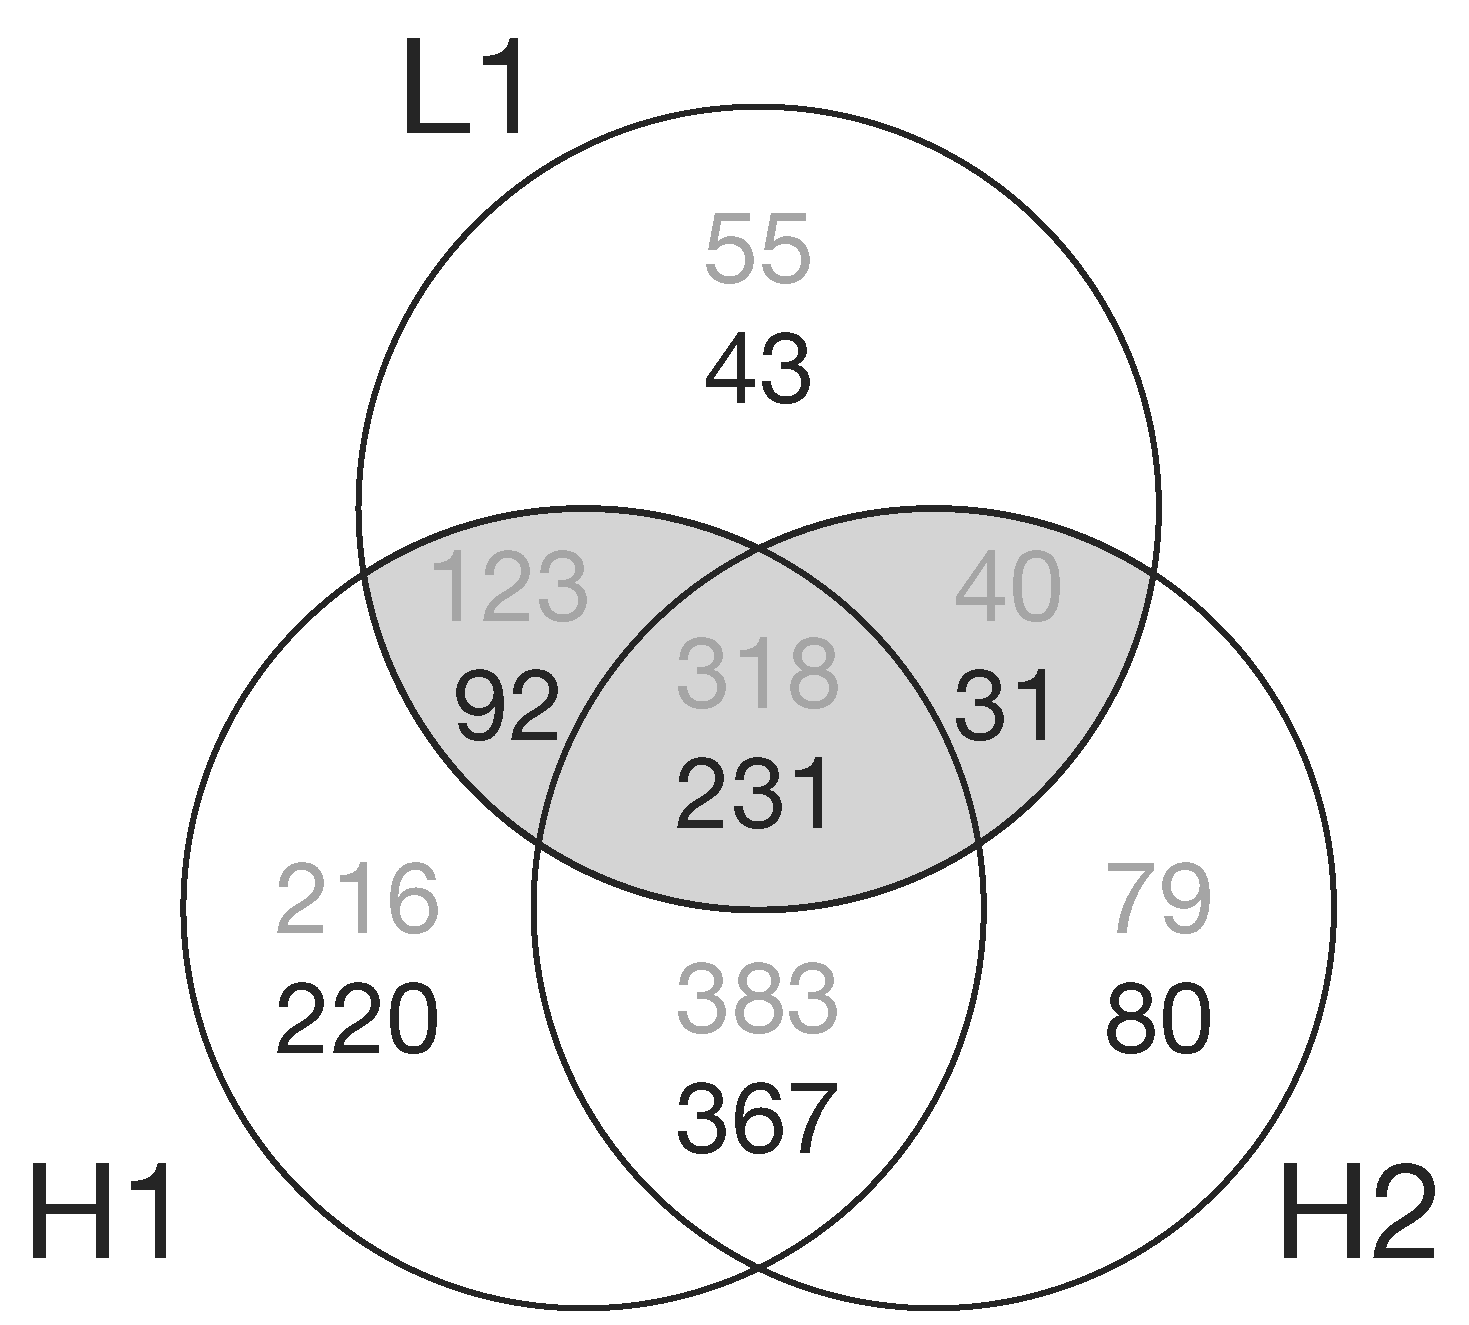
\includegraphics[width=\linewidth]{figures/result/s2_times}
\end{center}
\caption[Amounts of Single and Coincident Interferometer Data in S2]{%
\label{f:S2times}
The Venn diagram showns the number of hours that each detector combination was
operational during the S2 run.  The upper number gives the amount of time the
specific instruments were operational.  The lower number gives the total
non-playground time which was searched for inspiral triggers.  The shaded
region corresponds to the data used in the S2 MACHO search.}
\end{figure}

\begin{figure}[p]
\begin{center}
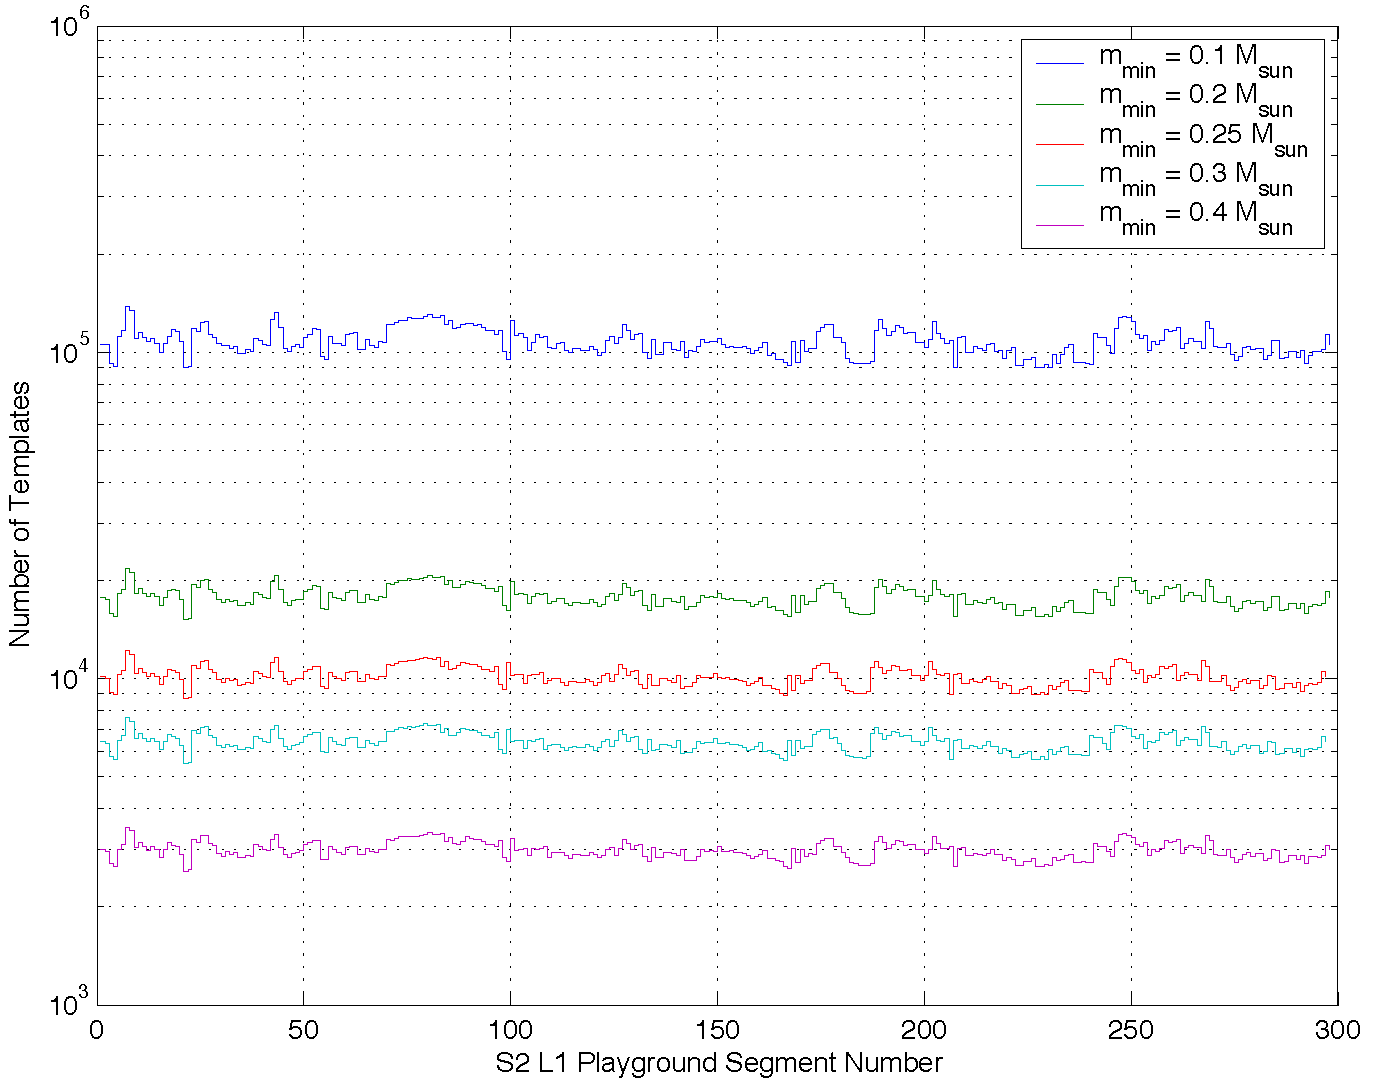
\includegraphics[width=\linewidth]{figures/result/bank_size}
\end{center}
\caption[MACHO Template Bank Size for Various Lower Masses]{%
\label{f:bank_size}
The plot shows the size of the template bank, generated with a minimal match
of $97\%$, for various values of $m_\mathrm{min}^{-8/3}$. As described in
section \ref{ss:templatebank} the size of the template bank is proportional to
$m_\mathrm{min}^{-8/3}$, where $m_\mathrm{min}$ is the mass parameter of the
smallest equal mass binary in the template bank. Using these data, it was
decided that the lowest mass accessible was $m_\mathrm{min} = 0.2\,M_\odot$,
given the available computational resources.}
\end{figure}

\begin{figure}[p]
\begin{center}
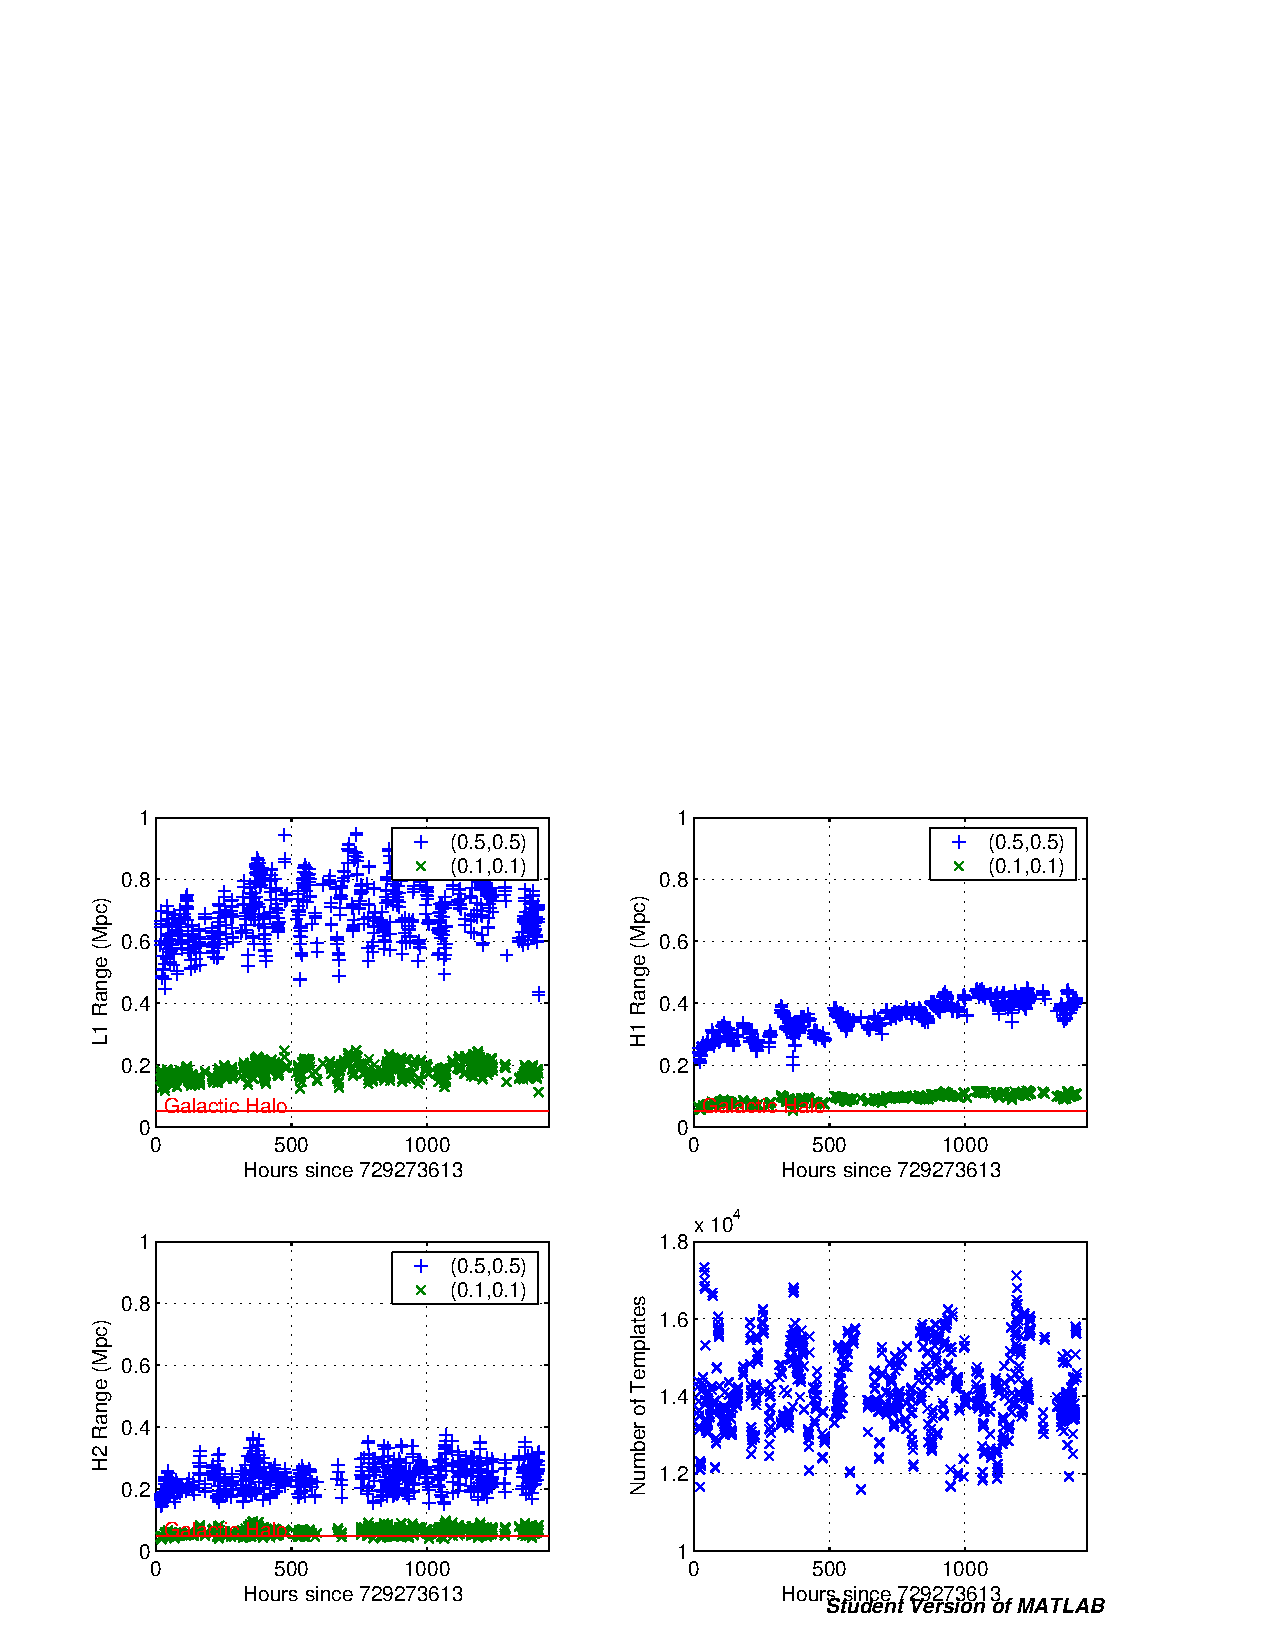
\includegraphics[width=\linewidth]{figures/result/s2_macho_range_summary}
\end{center}
\caption[S2 Inteferometer Ranges and Template Bank Size]{%
\label{f:inspiral_summary}
The bottom right plots shows the variation in the size of the MACHO search
template bank over the course of the S2 run. As described in the text, the
template bank is generated using L1 data to cover a region of parameter space
from $0.2\,M_\odot$ to $1.0\,M_\odot$ (component mass) at $95\%$ minimal
match. This template bank is used to filter the L1 data in the triggered
search pipeline. The other three plots show the variation in distance to which
the three LIGO interferometers can see an optimally oriented binary at
signal-to-noise ratio 8 over the S2 run. Since this is a function of the
masses of the binary, this range is shown for a $(0.1,0.1)\,M_\odot$ and a
$(0.5,0.5)\,M_\odot$ binary.
}
\end{figure}

\begin{figure}[p]
\begin{center}
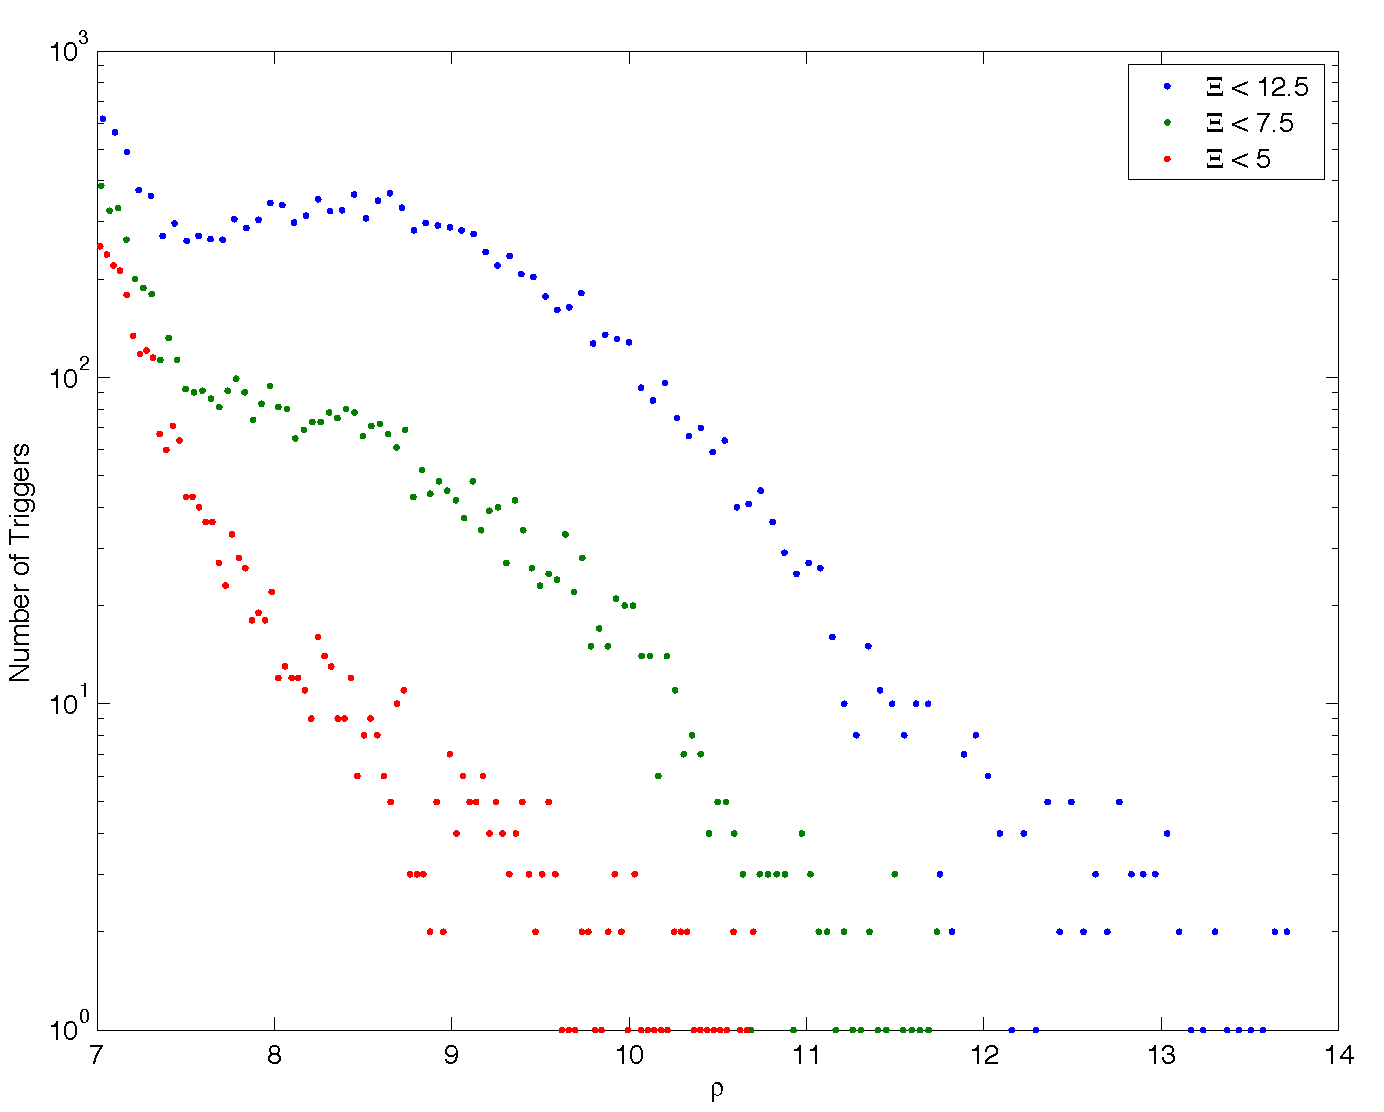
\includegraphics[width=\textwidth]{figures/result/h1l1_snr_hist_delta_0_04_chisq_12_5}
\end{center}
\caption[Tuning the $\chi^2$ Veto for H1]{%
\label{f:h1_chisq_tuning}
The figure shows a histogram of all the triggers generated from the H1 data
using the triggered search (i.e. no coincidence with L1 or H2 has been applied
to the triggers). The signal-to-noise threshold is $\rho_\ast = 7$ and the
parameters of the $\chi^2$ veto are $p = 15, \delta^2 = 0.04, \Xi = 12.5$, as
in the S2 binary neutron star search. If the interferometer data is Gaussian,
then we would expect the histogram to be monotonically decreasing with
increasing signal-to-noise ratio, however there is a pronouced ``hump'' in the
histogram at $\rho\approx 9$ suggesting some non-Gaussian feature in the data.
By lowering the value of $\Xi$ to $5$, we can remove this feature from the
histogram, but we must be careful in doing so that we do not reduce the
detection efficiency of the pipeline.
}
\end{figure}

\begin{figure}[p]
\begin{center}
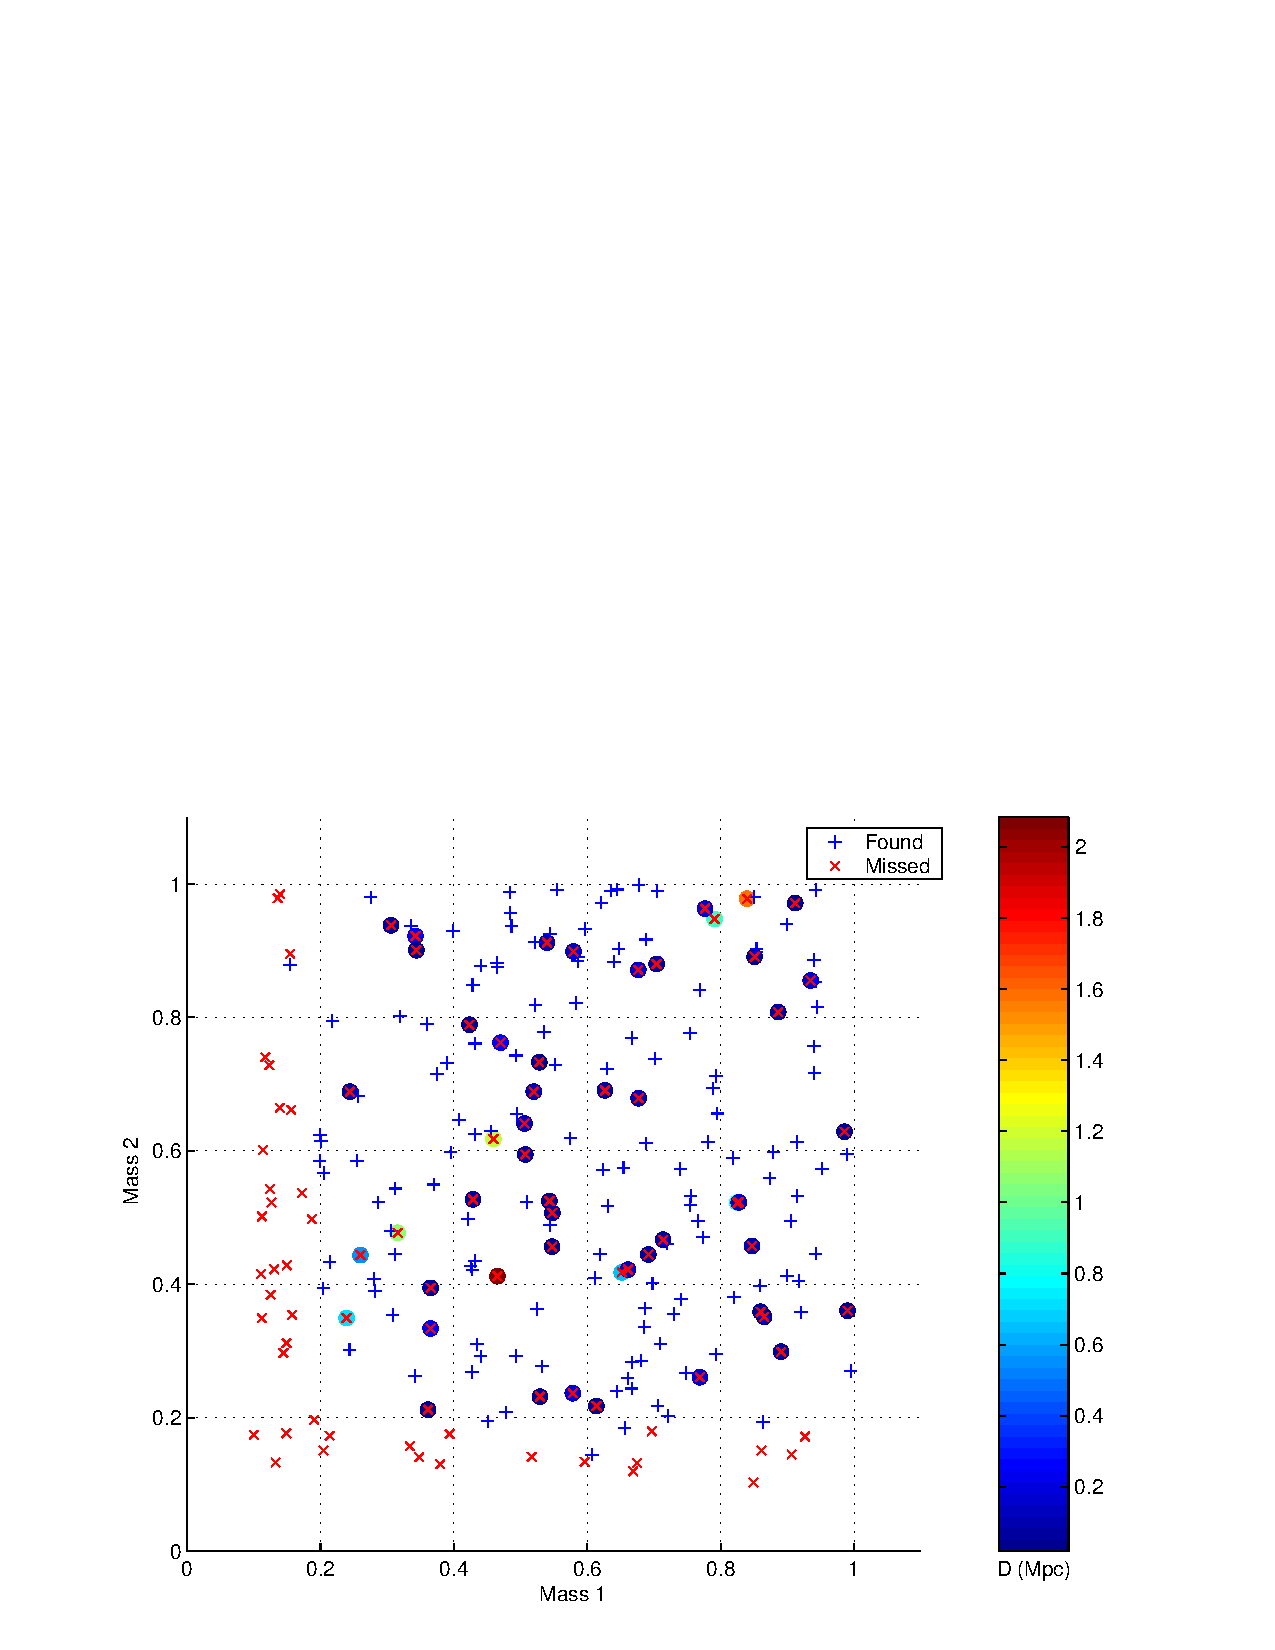
\includegraphics[width=\textwidth]{figures/result/h1_inj_mass_7_0_delta_0_04_chisq_12_5}
\end{center}
\caption[Found and Missed H1 Injections for $\Xi = 12.5 \delta^2 = 0.04$]{%
\label{f:h1_missed_tuning}
The figure shows the results of a small Monte Carlo simulation used to test
the detection efficiency of the pipeline using H1 triggers (i.e. no
coincidence with L1 or H2 has been applied to the triggers). The
signal-to-noise threshold is $\rho_\ast = 7$ and the parameters of the
$\chi^2$ veto are $p = 15, \delta^2 = 0.04, \Xi = 12.5$. Found injections are
shown with a $+$, missed injections are shown with a $\times$ and the masses
of the injection are shown as the $x$ and $y$ coordinates. We would expect to
miss any injections with a mass component below $0.2\,M_\odot$ due to the
covereage of the template bank, however injections in the region inside the
bank should be detected, unless they are at an effective distance larger than
the range of the interferometer. The missed injections that we would expect to
find are color coded according to the effective distance at which they are
injected.  Several injections are missed as they are at a large effective
distance (e.g.  the injection at $(0.48,0.42)\,M_\odot$), however there are
may missed injections at distances $< 200$~kpc which should be detectable in
the H1 data (e.g. the injection at $(0.88,0.91)\,M_\odot$. Investigation of
the missed injections showed that although they had large values of
signal-to-noise This suggests that
the search parameters used must be re-tuned to increase the detection
efficiency.
}
\end{figure}

\begin{figure}[p]
\begin{center}
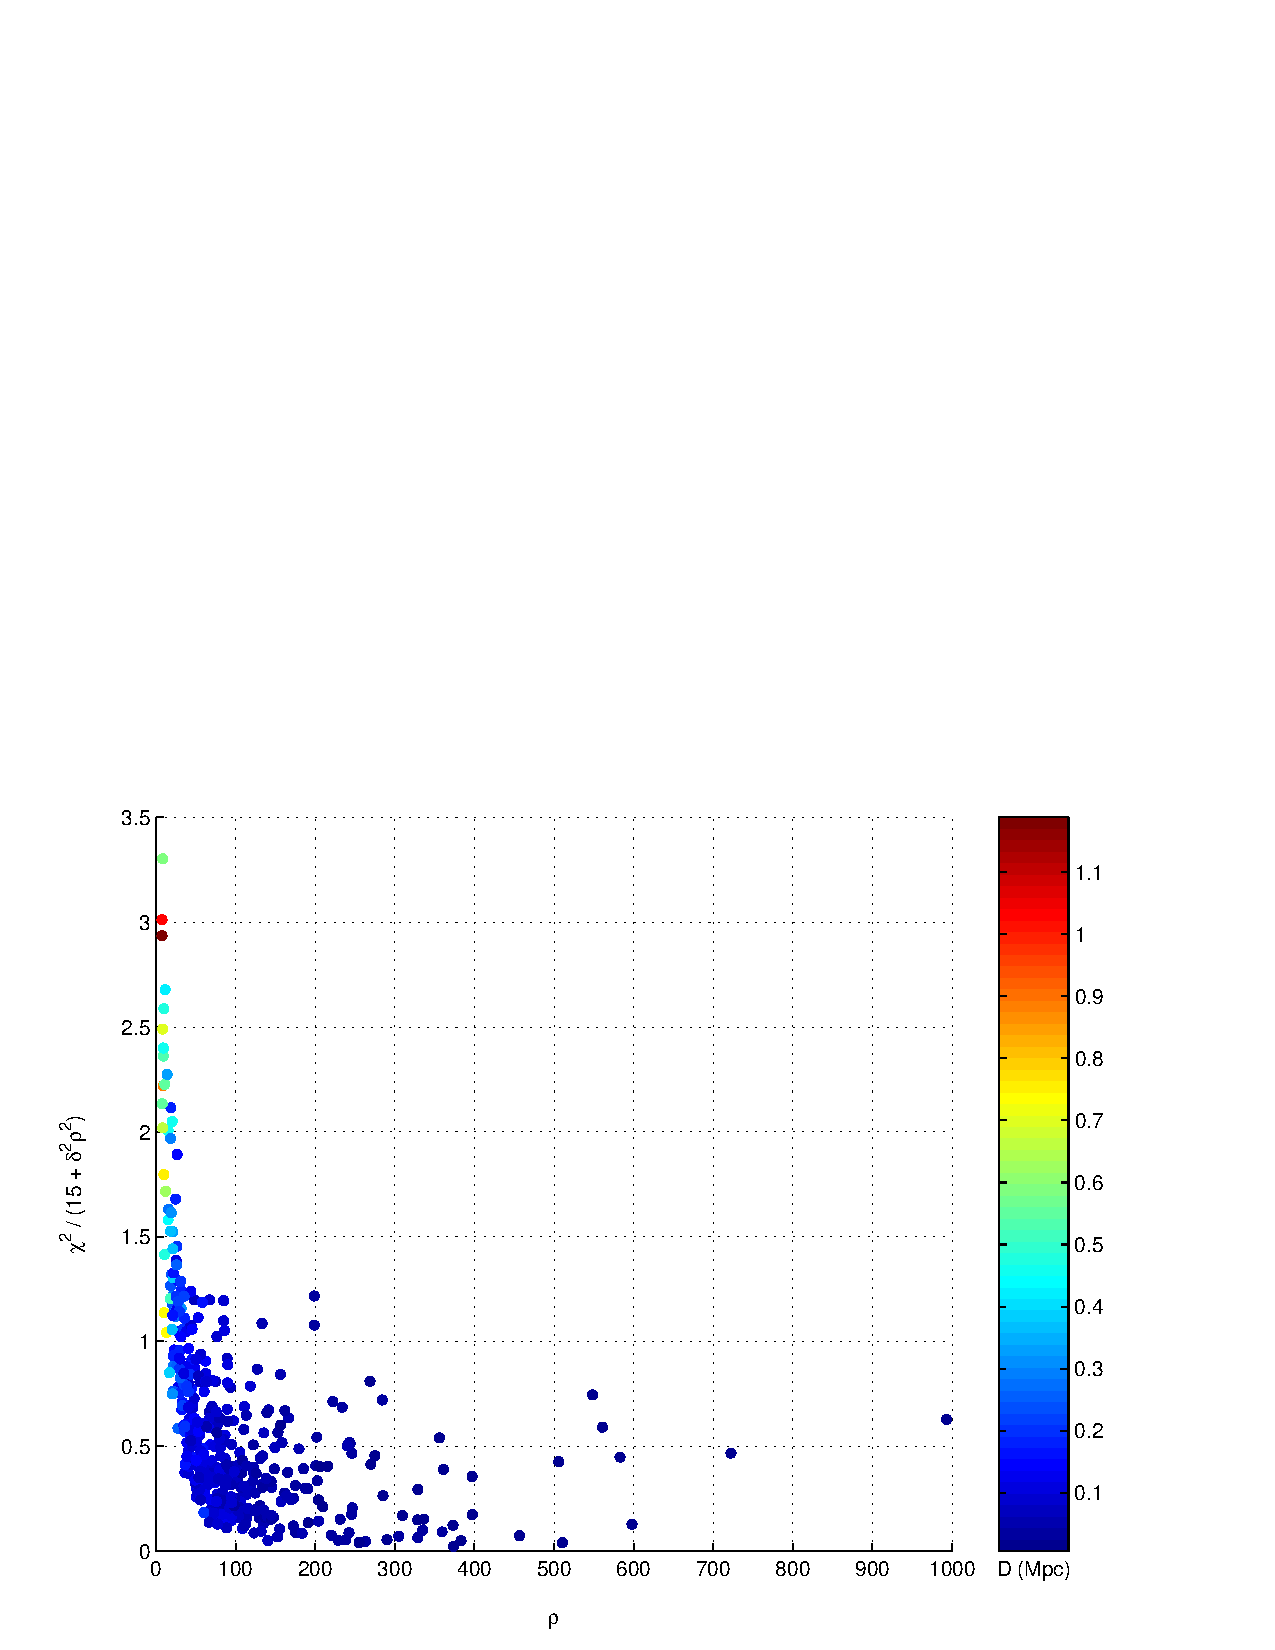
\includegraphics[width=0.7\textwidth]{figures/result/l1_inj_snr_7_0_delta_0_04_chisq_5_0}\\
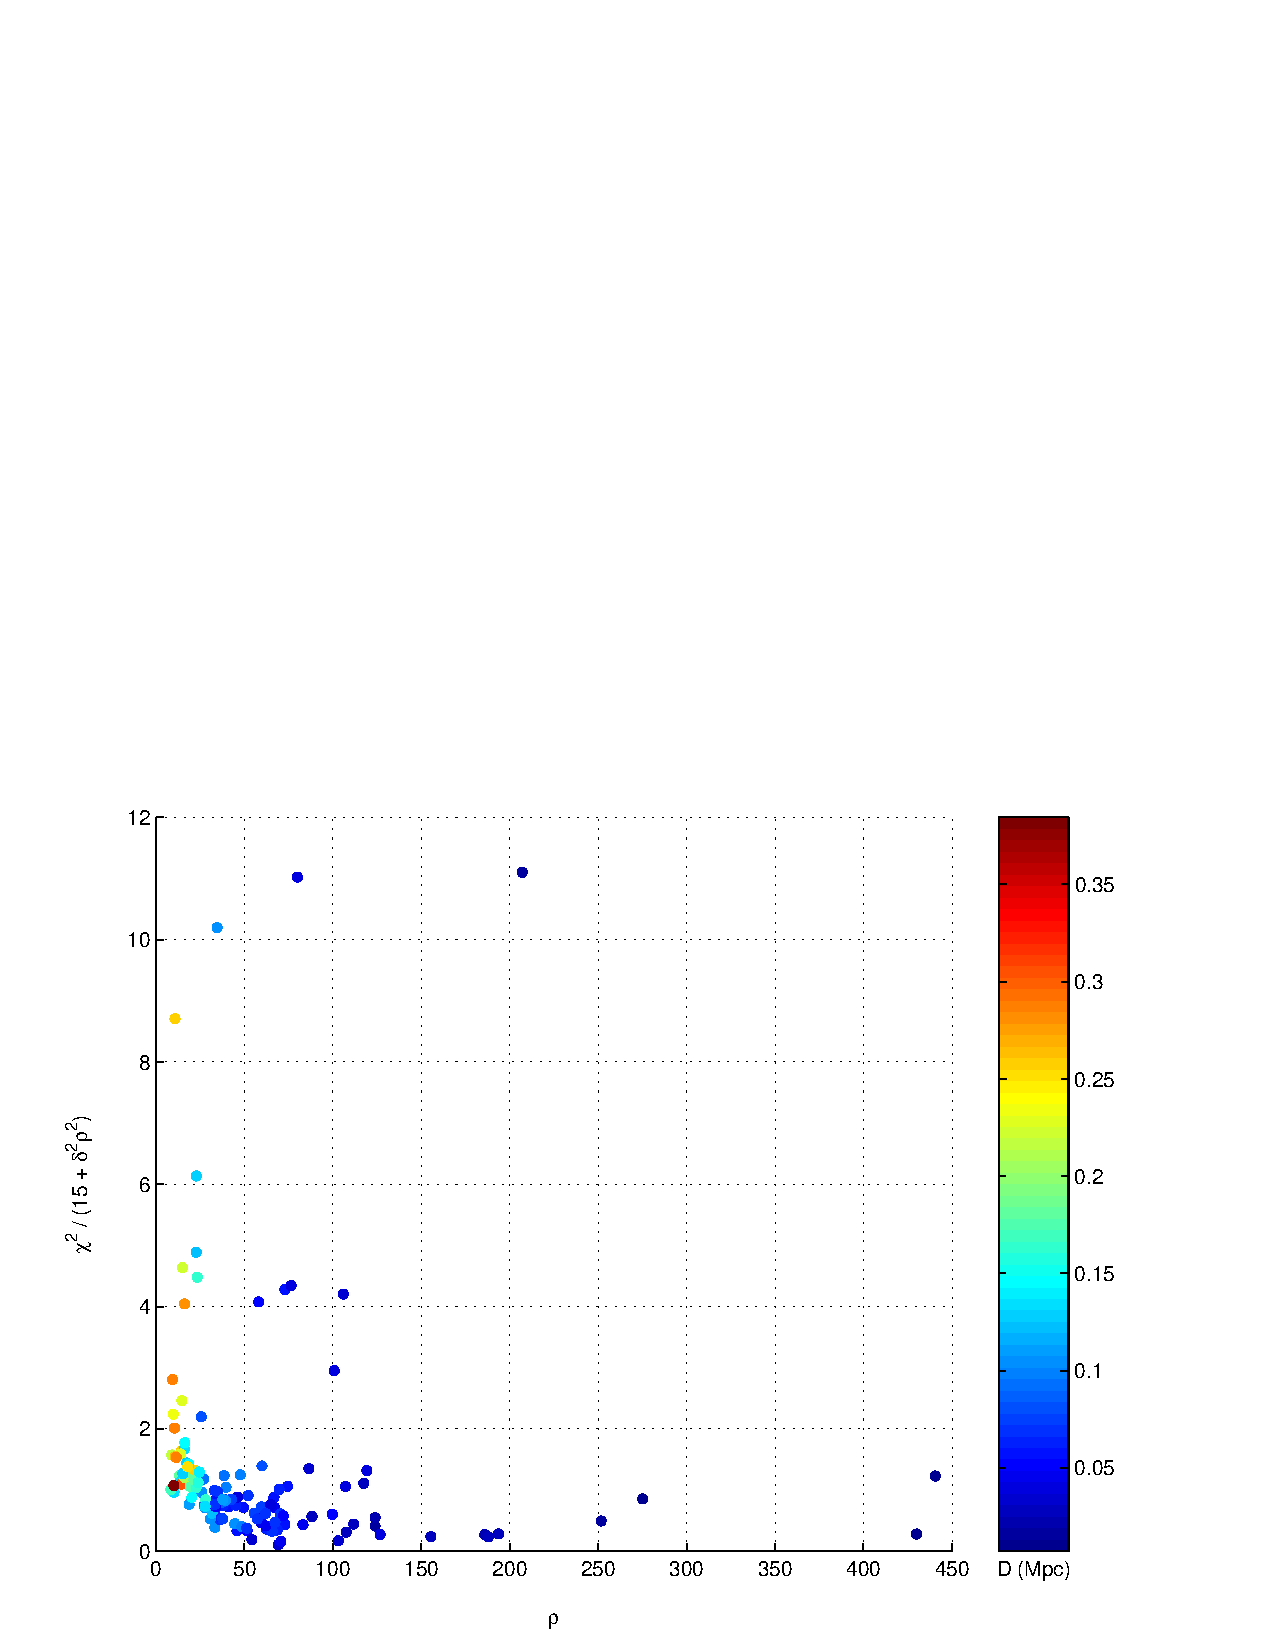
\includegraphics[width=0.7\textwidth]{figures/result/h1_inj_snr_7_0_delta_0_04_chisq_12_5}
\end{center}
\caption[Illustration of Tuning Based on Injections]{%
\label{f:h1_inj_xi_tuning}
The plots in this figure show the values of $\rho$ and $\chi^2/(15 +
\delta^2\rho^2)$ for the inspiral triggers corresponding to injected signals
found by the triggered search pipeline. The upper plot shows L1 triggers and
the lower plot shows H1 triggers (which correspond to the found injections of
figure \ref{f:h1_missed_tuning}). No coincidence has been applied to the H1
triggers at this stage, however they are generated using template banks
produced from L1 triggers. The color of each trigger shows the effective
distance at which it was injected.  Both plots are generated with a
signal-to-noise threshold of $\rho_\ast = 7$ and the parameters of the
$\chi^2$ veto were $p = 15, \delta^2 = 0.04$ and $\Xi_\mathrm{L1} = 12.5,
\Xi_\mathrm{L1} = 5.0$, values chosen based on the tuning of the S2 binary
neutron star search. It can be seen that, at a given signal-to-noise ratio,
the H1 triggers typically have higher values of $\Xi$ than the L1 triggers.
This is due to the a larger mismatch between the injected signal and the
templates in the H1 triggered bank.
}
\end{figure}

\begin{figure}[p]
\begin{center}
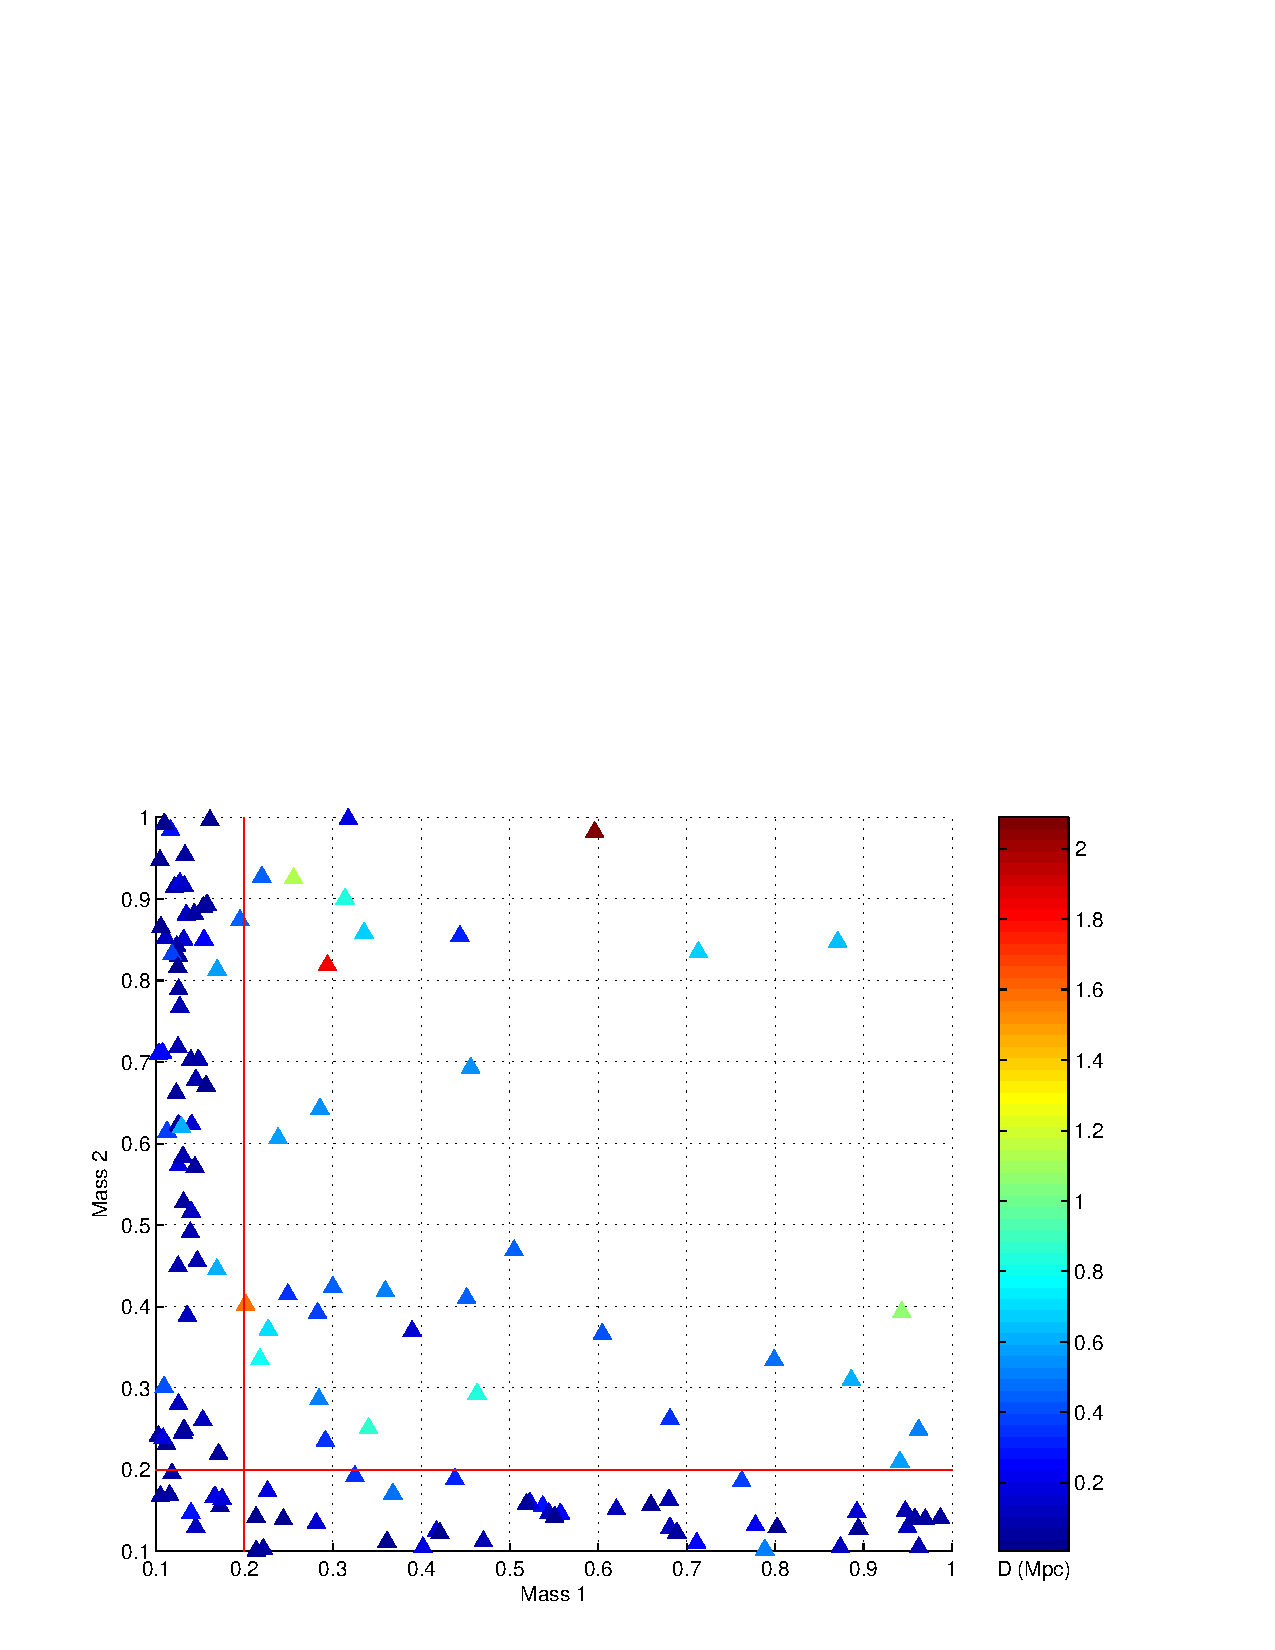
\includegraphics[width=\textwidth]{figures/result/m1m2_missed}
\end{center}
\caption[Simulated Signals Not Detected by Pipeline]{%
\label{f:m1m2_missed}
Found injections.
}
\end{figure}

\begin{figure}[p]
\begin{center}
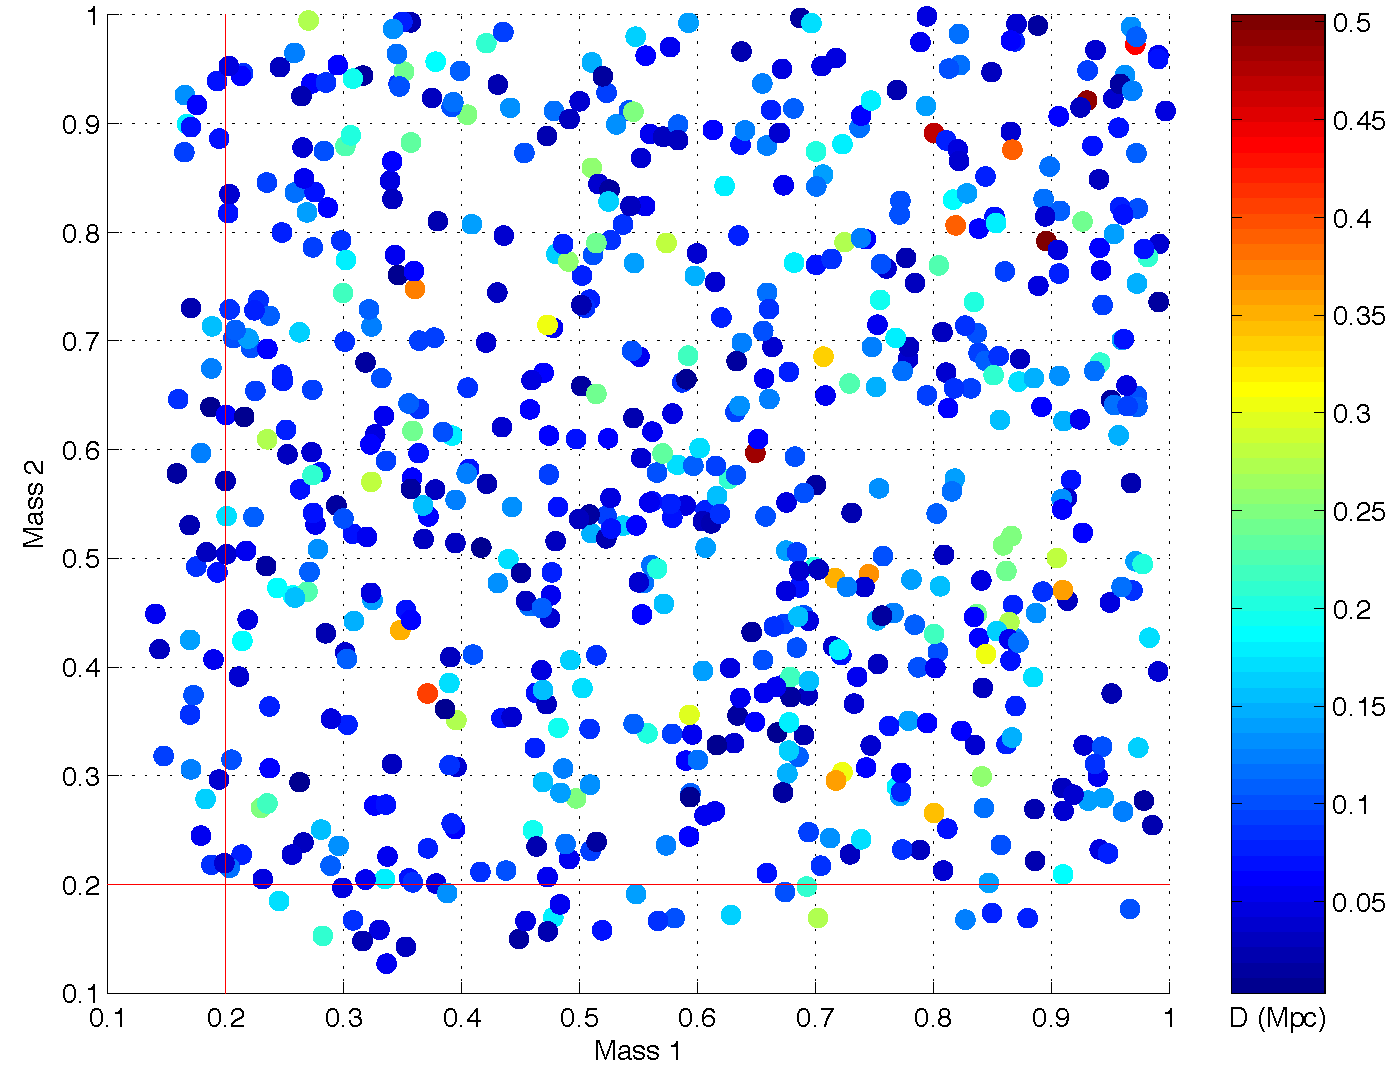
\includegraphics[width=\textwidth]{figures/result/m1m2_found}
\end{center}
\caption[Simulated Signals Detected by Pipeline]{%
\label{f:m1m2_found}
Found injections.
}
\end{figure}

\begin{figure}[p]
\begin{center}
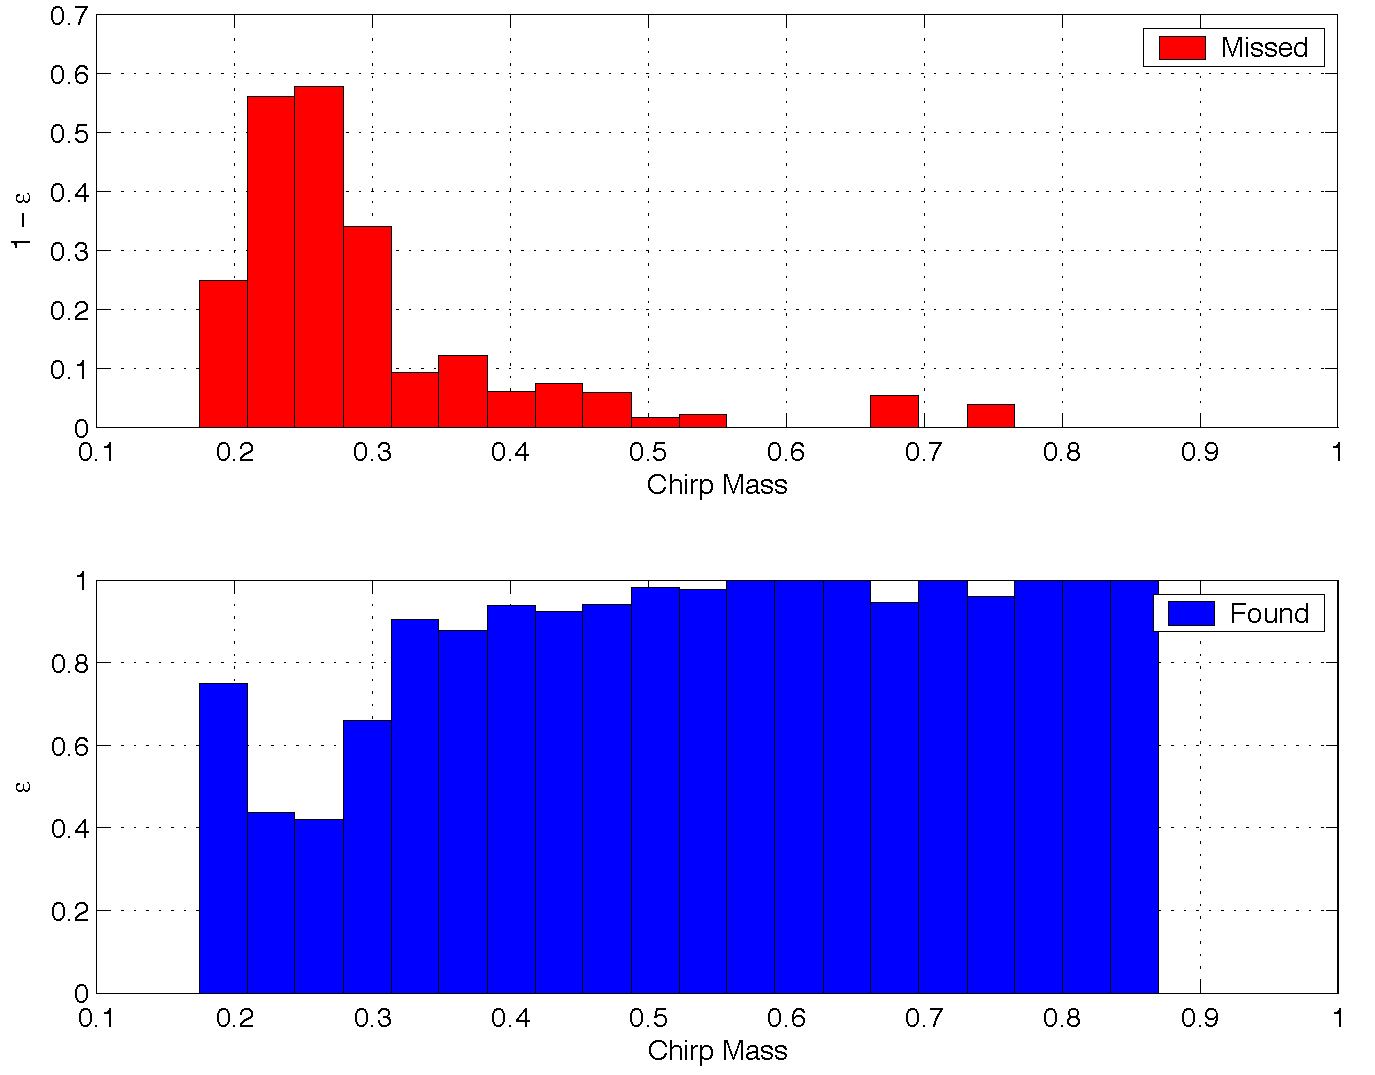
\includegraphics[width=0.7\textwidth]{figures/result/mchirp_eff} \\
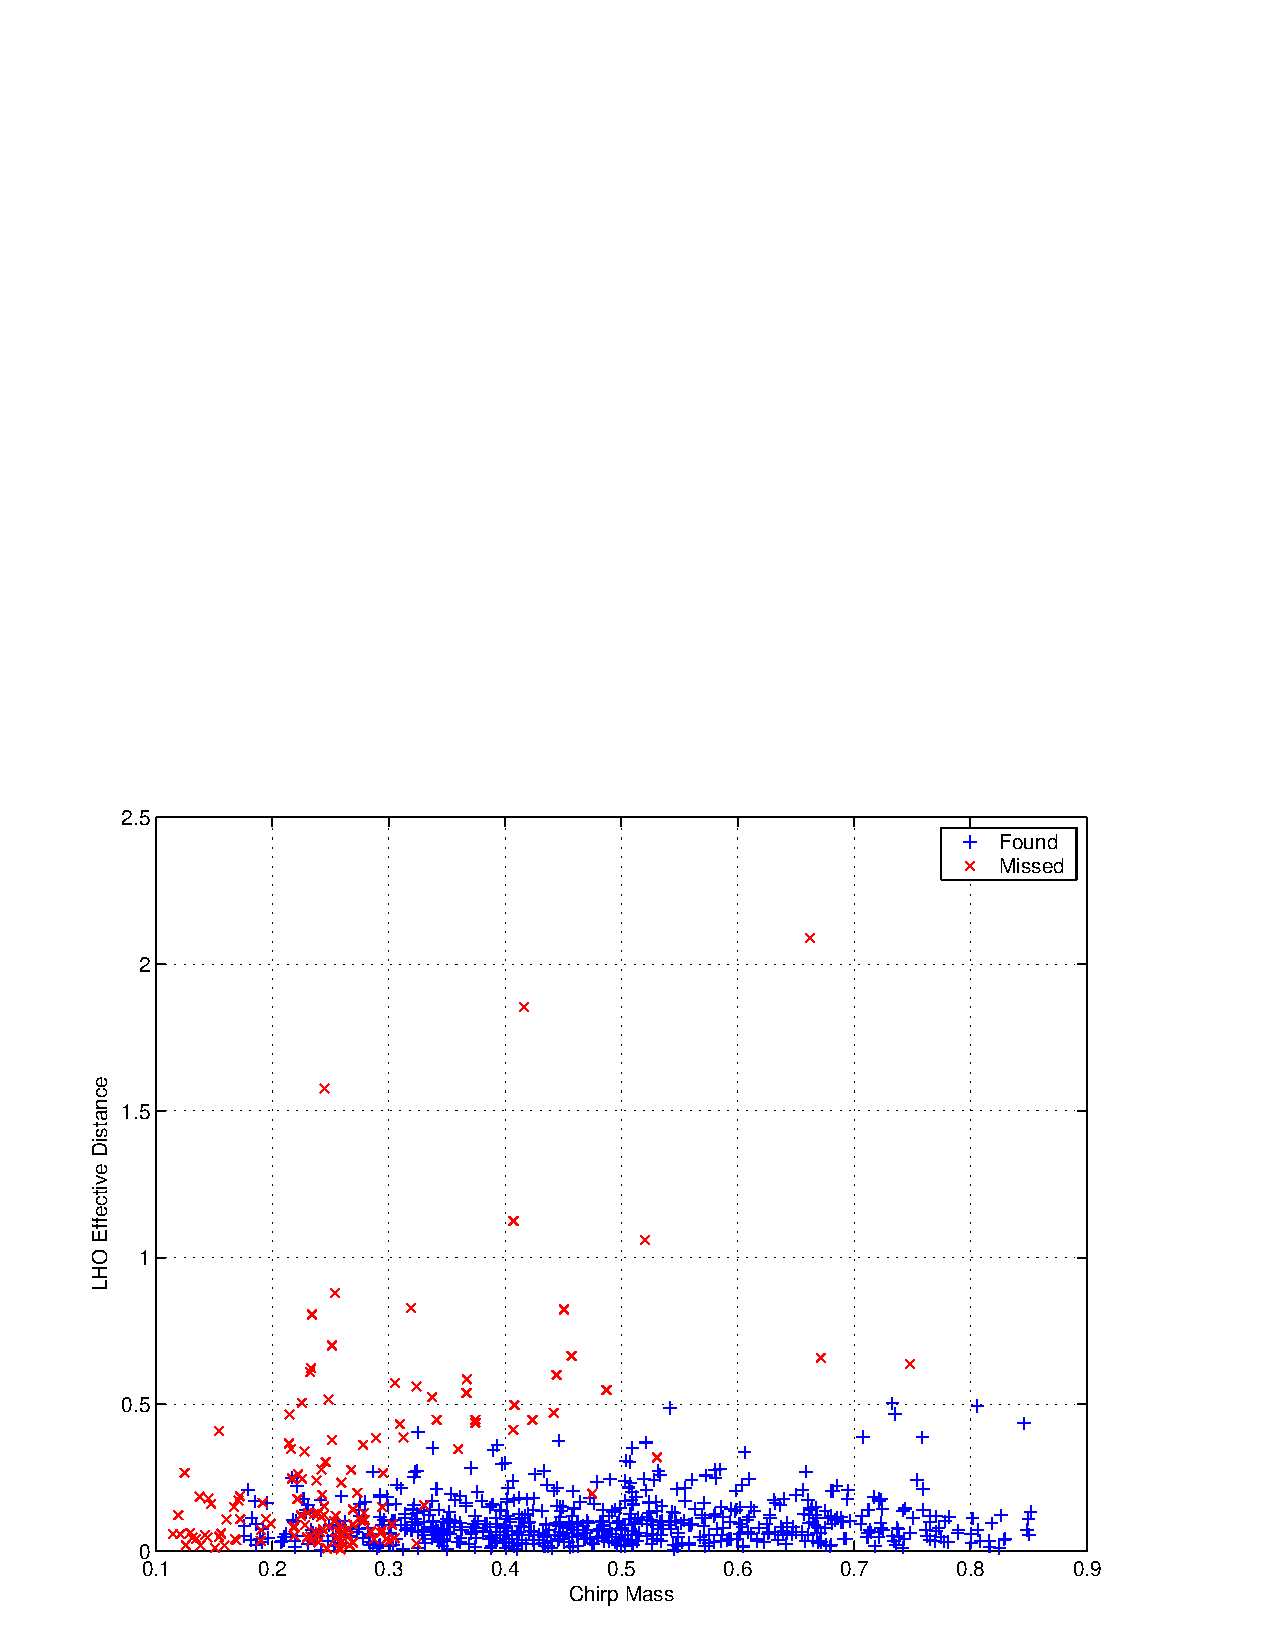
\includegraphics[width=0.7\textwidth]{figures/result/mchirp_found_missed}
\end{center}
\caption{\label{f:mchirp_eff}%
Found injections.
}
\end{figure}

\begin{figure}[p]
\begin{center}
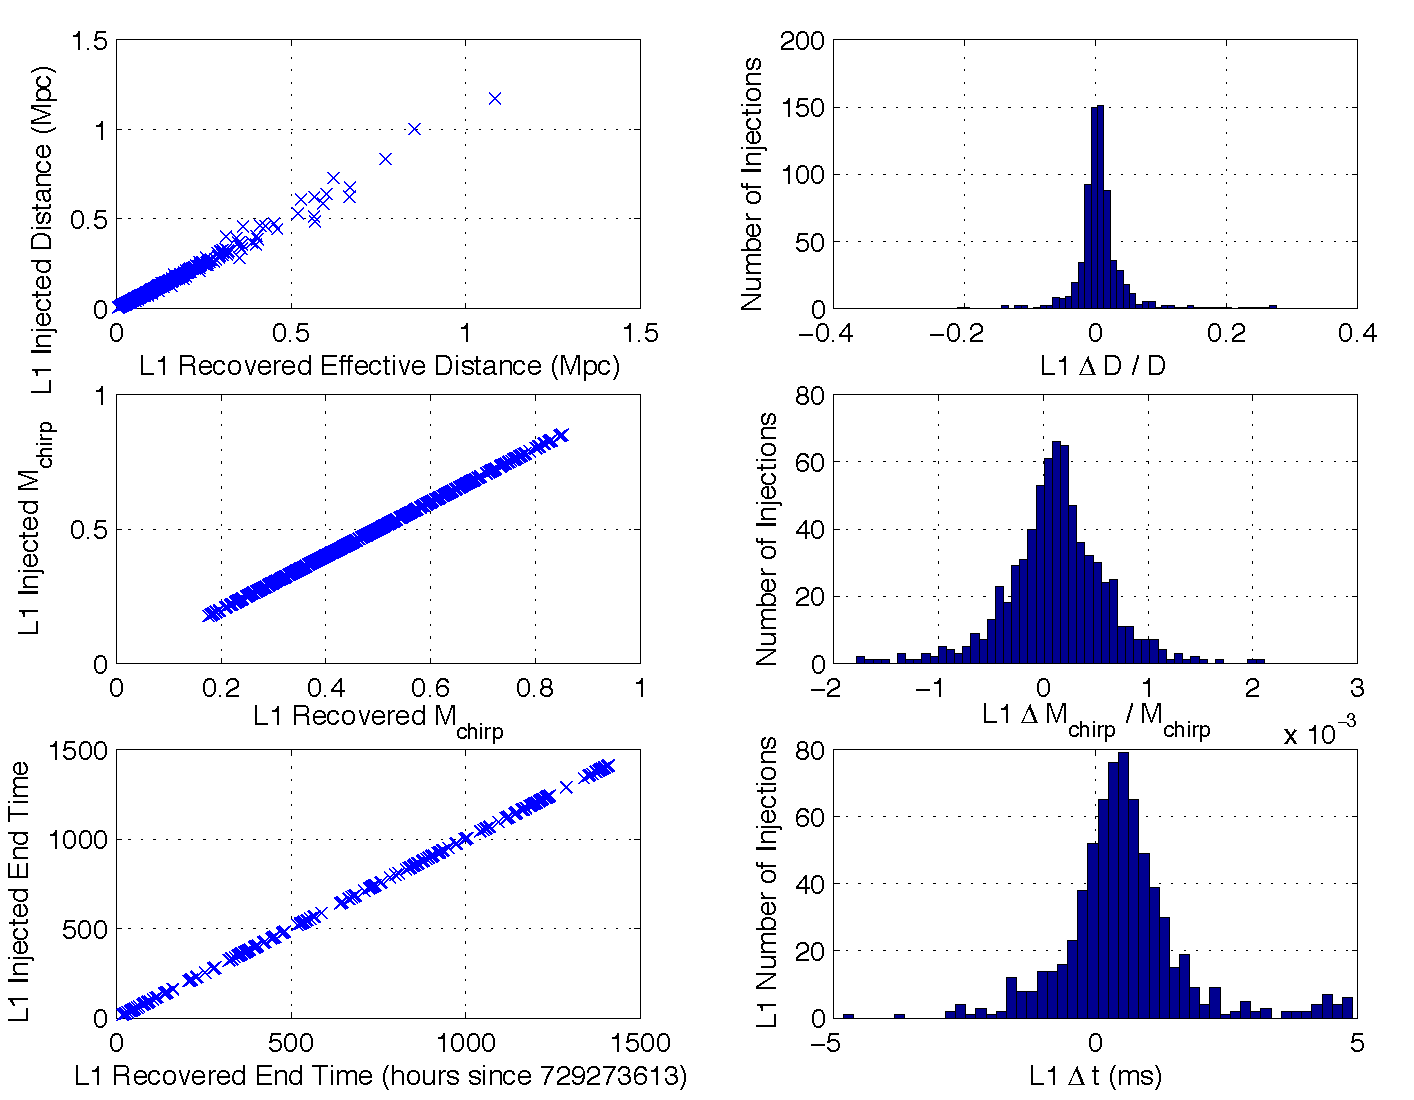
\includegraphics[width=\textwidth]{figures/result/l1_param_error}
\end{center}
\caption{\label{f:l1_param_error}%
Found injections.
}
\end{figure}

\begin{figure}[p]
\begin{center}
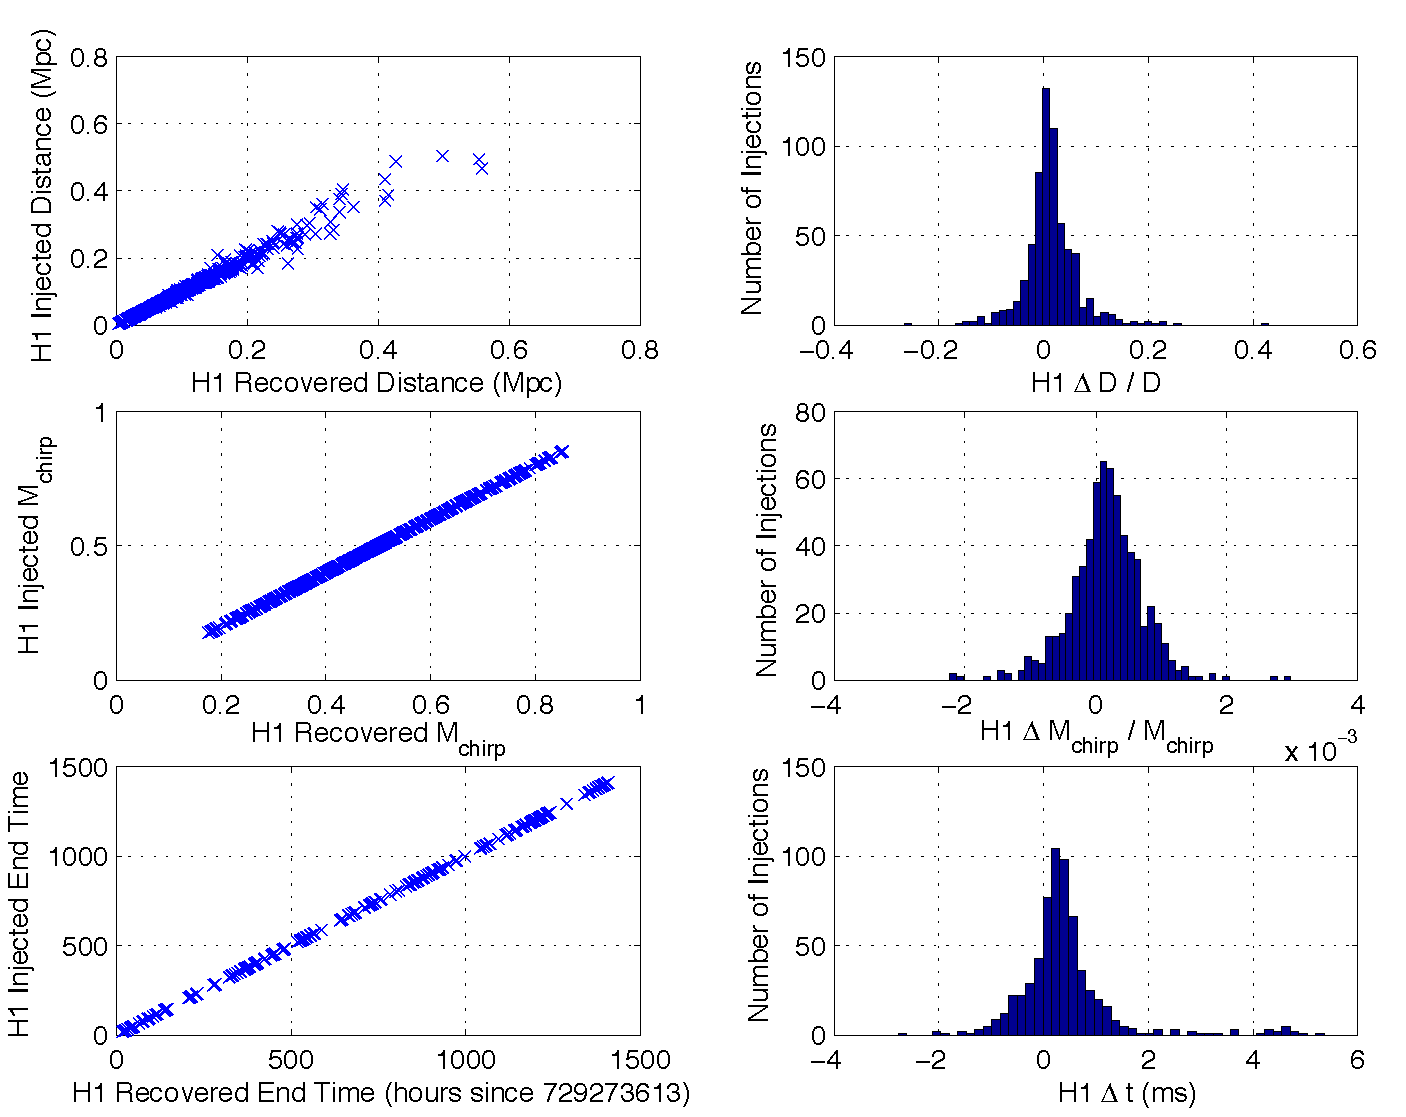
\includegraphics[width=\textwidth]{figures/result/h1_param_error}
\end{center}
\caption{\label{f:h1_param_error}%
Found injections.
}
\end{figure}

\begin{figure}[p]
\begin{center}
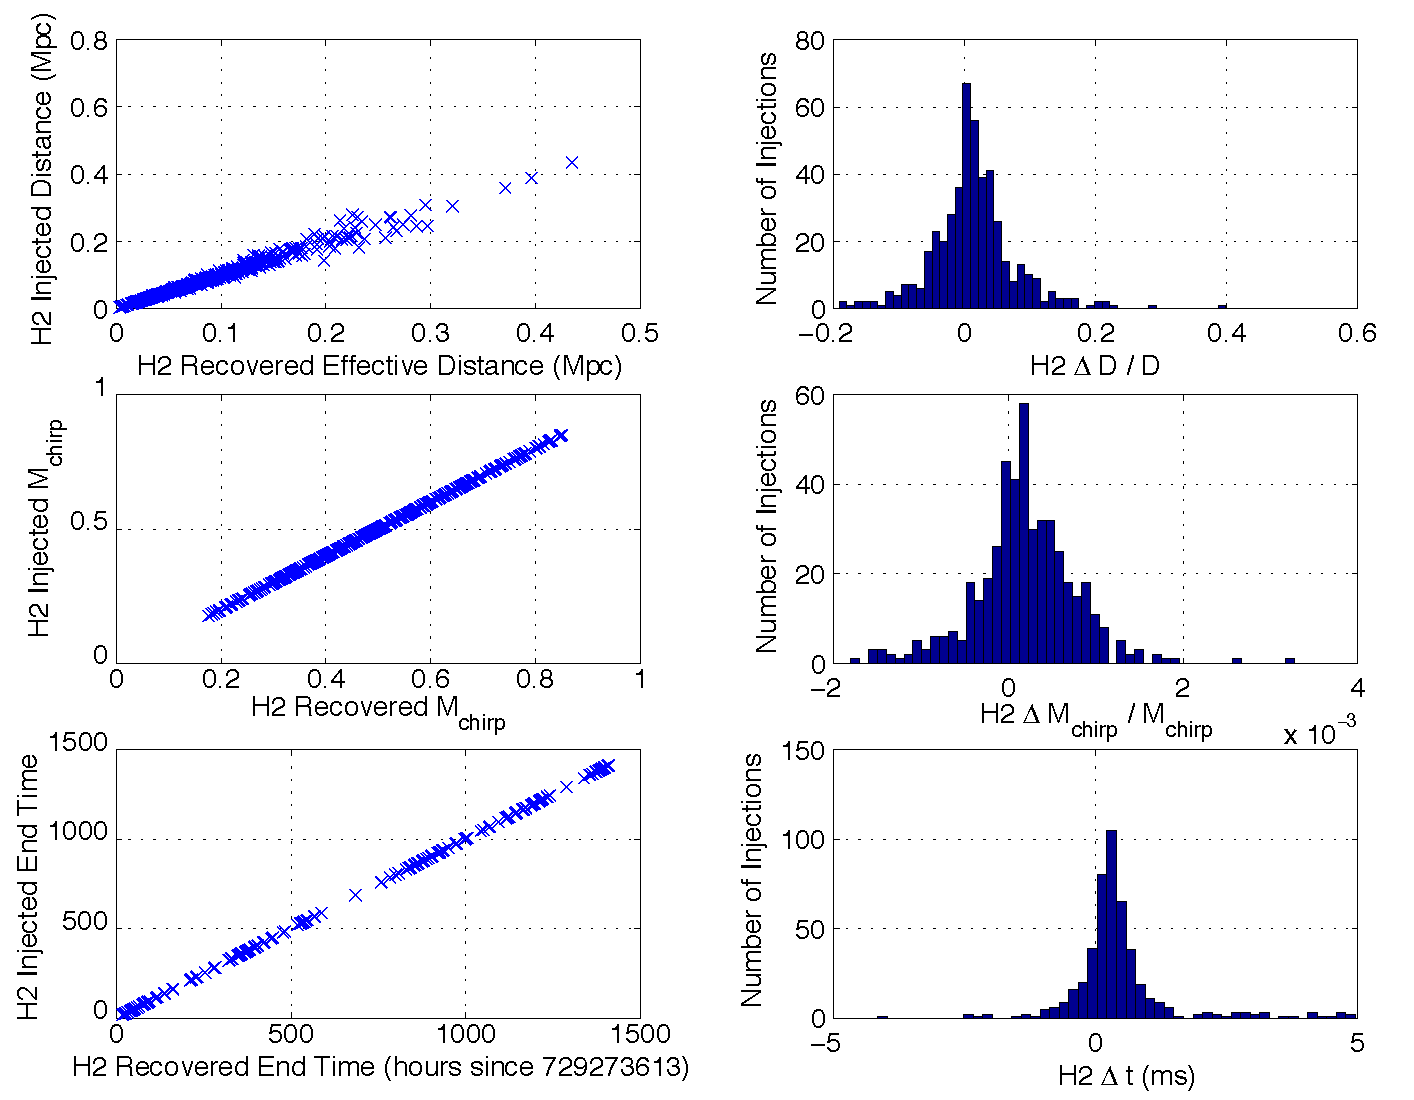
\includegraphics[width=\textwidth]{figures/result/h2_param_error}
\end{center}
\caption{\label{f:h2_param_error}%
Found injections.
}
\end{figure}

\begin{figure}[p]
\begin{center}
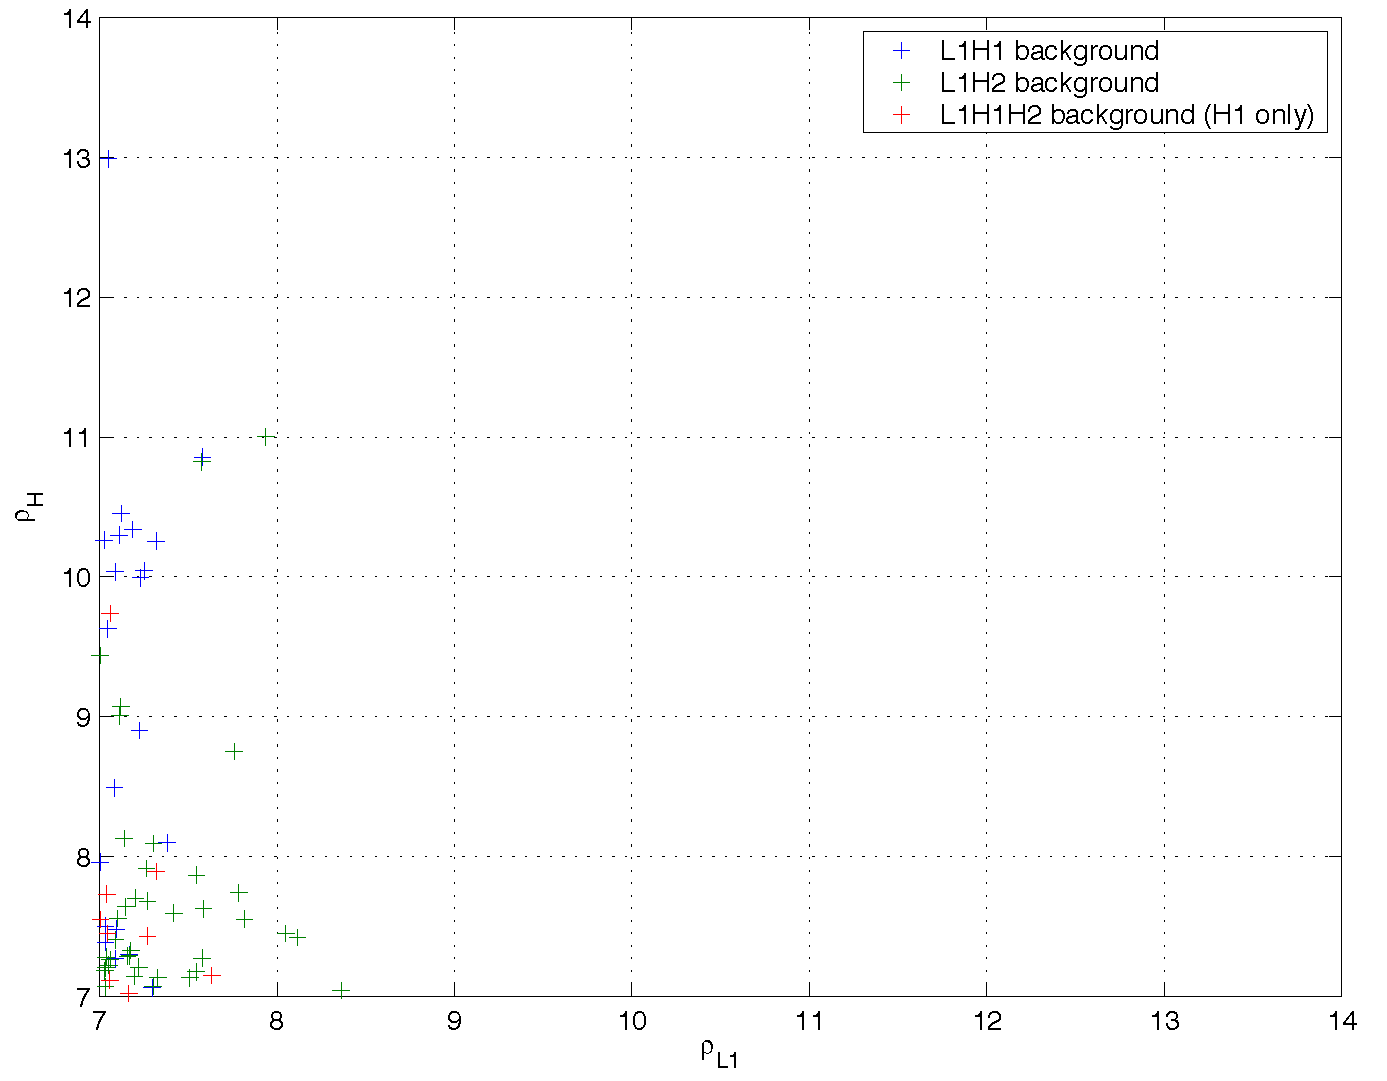
\includegraphics[width=\textwidth]{figures/result/bkg}
\end{center}
\caption{\label{f:inj_bkg_snr}%
Found injections.
}
\end{figure}

\begin{figure}[p]
\begin{center}
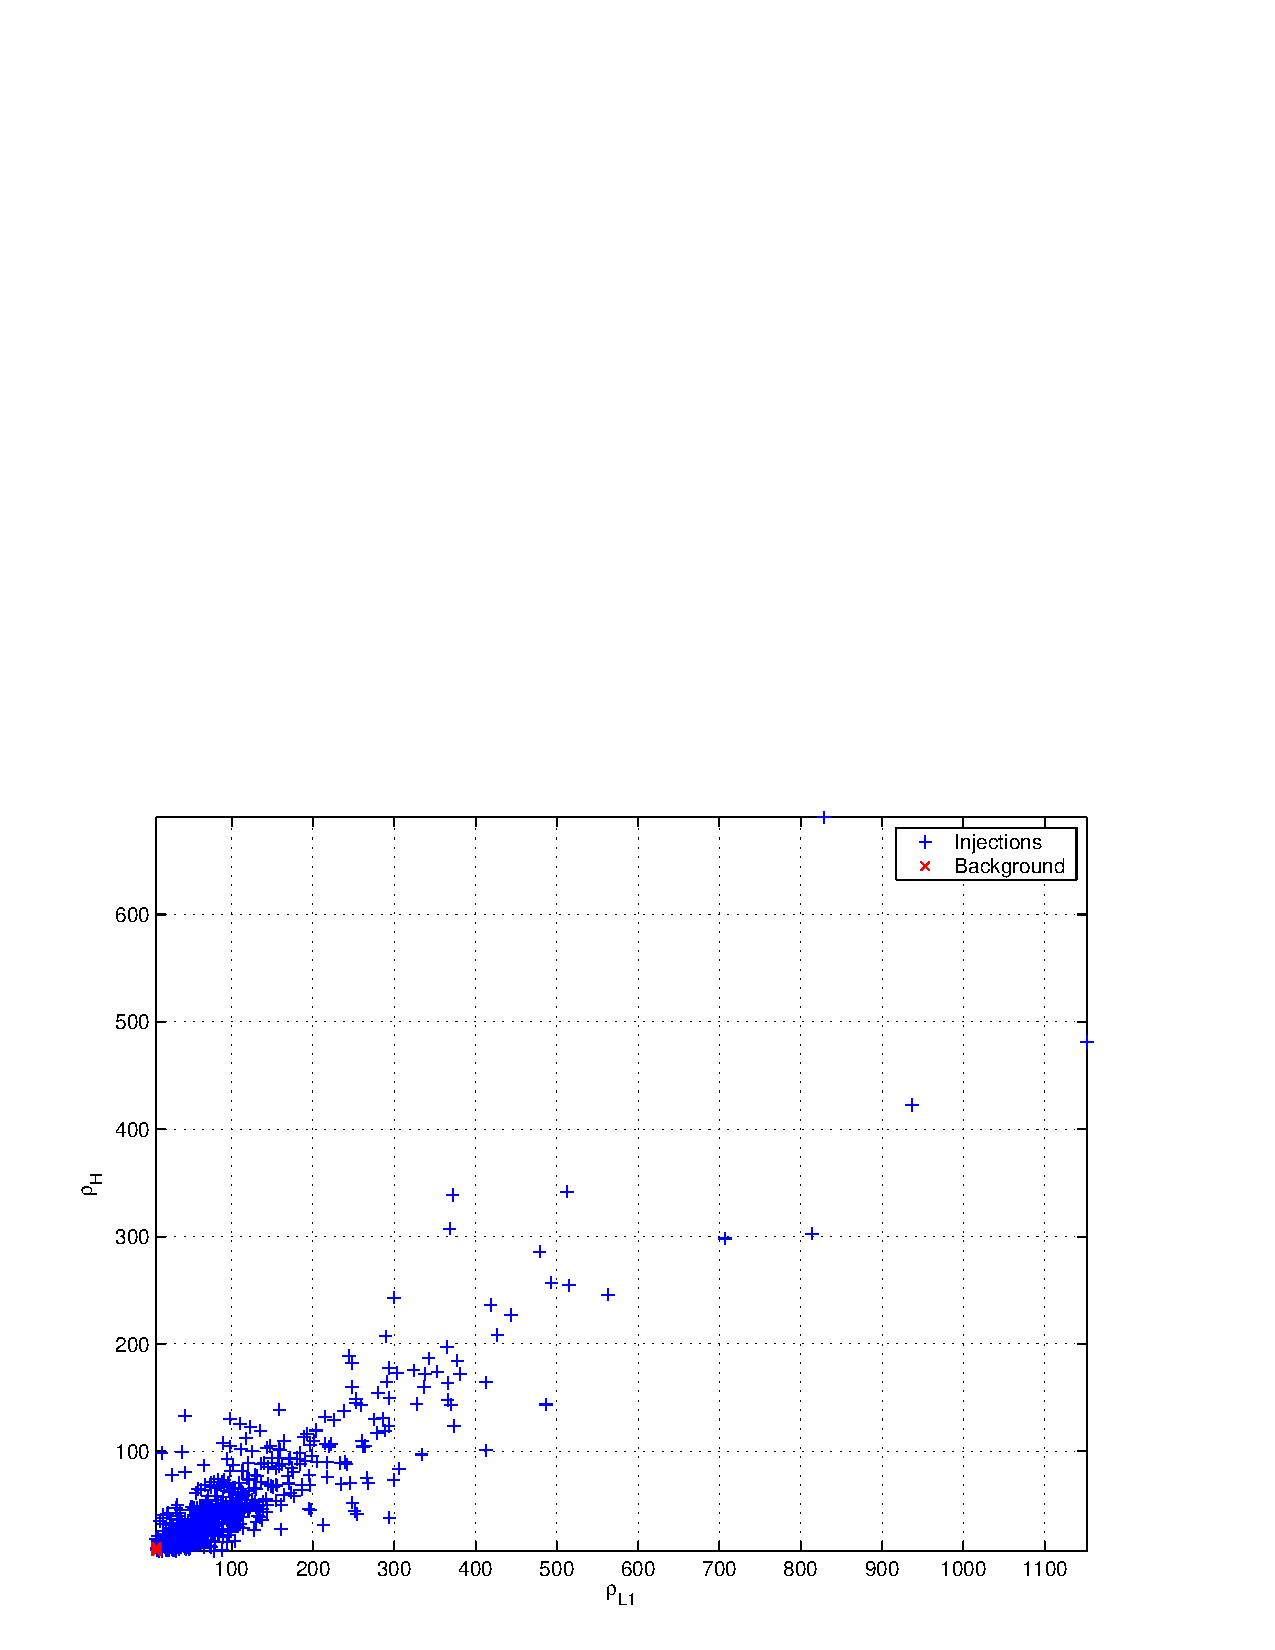
\includegraphics[width=\textwidth]{figures/result/bkg_inj}
\end{center}
\caption{\label{f:bkg_hist}%
Found injections.
}
\end{figure}

\begin{figure}[p]
\begin{center}
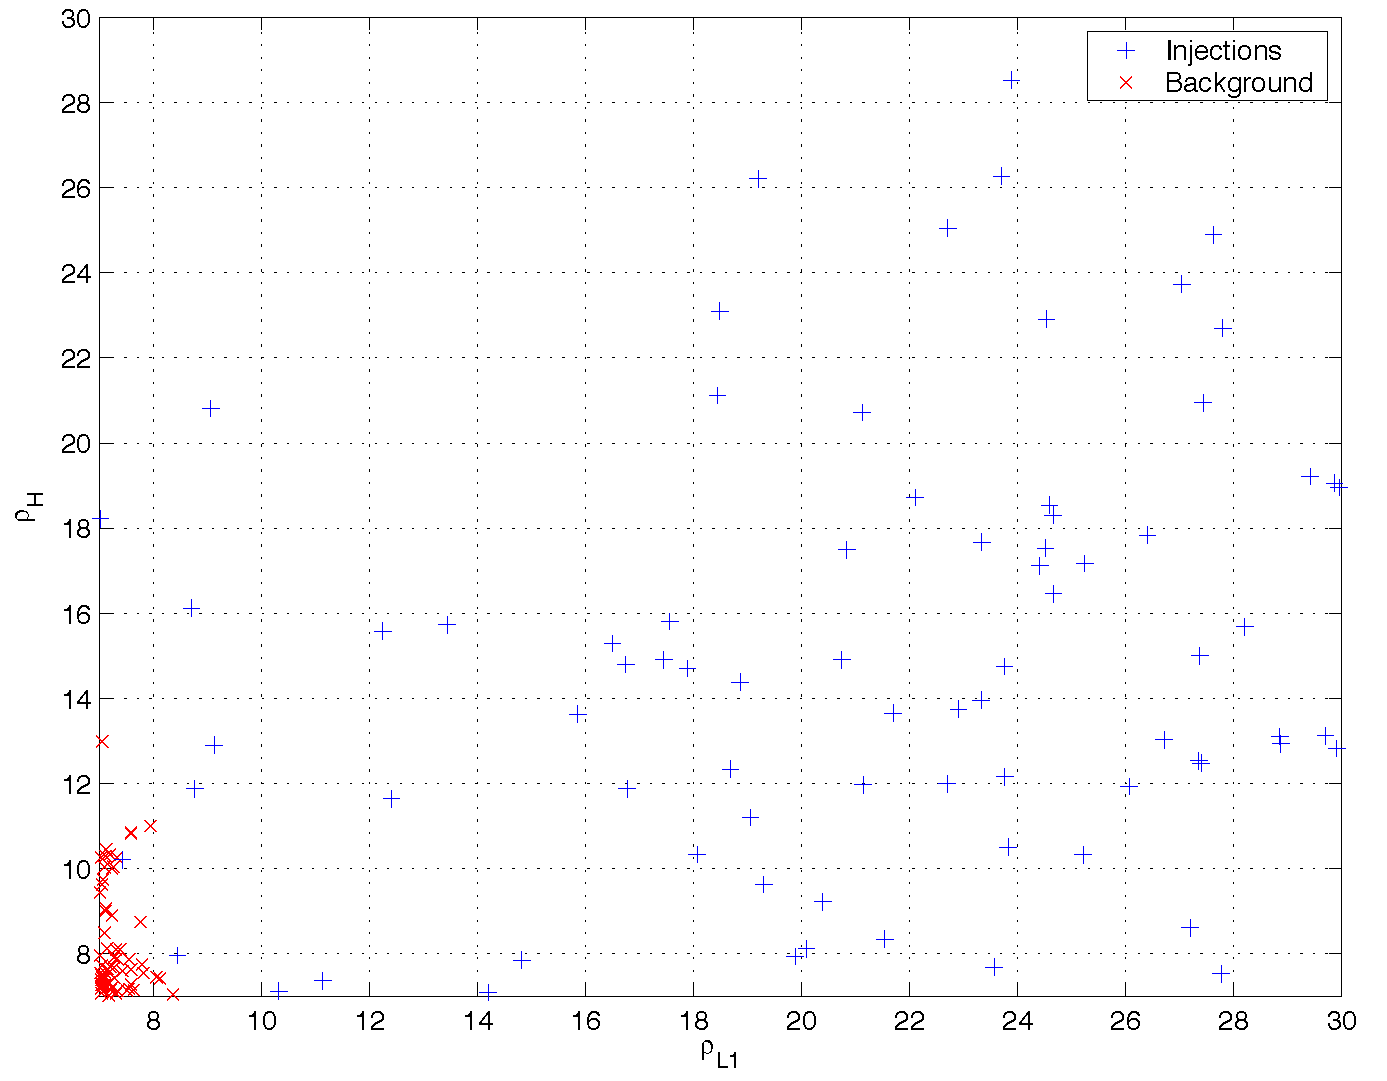
\includegraphics[width=\textwidth]{figures/result/bkg_inj_zoom}
\end{center}
\caption{\label{f:bkg_hist}%
Found injections.
}
\end{figure}

\begin{table}
\caption{\label{t:ifo_params}%
A complete list of the parameters that were selected at the various
stages of the pipeline.   These cuts are justified in the text.
}
\begin{tabular}{clr}
Parameter & Pipeline node & value \\
\hline 
$\rho^\ast_L$ & L1 GW Data & 6.0 \\
$\chi^2_L$ & L1 GW Data & 5.0 \\
$\rho^\ast_H$ & H1/H2 GW Data & 6.0 \\
$\chi^2_H$ & H1/H2 GW Data & 12.5 \\
$\delta m$ & Trigger Coincidence (all) & 0.0 \\
$\delta t$ & H1/H2 Trigger Coincidence & 0.001 s \\
$\delta t$ & L1/H1 and L1/H2 Trigger Coincidence & 0.011 s \\
$\kappa_{HH}$ & H1-H2 Coincidence & 0.5 \\
$\epsilon_{HH}$ & H1-H2 Coincidence & 2
\end{tabular}
\end{table}




